\documentclass[sigconf]{acmart}

\usepackage{booktabs} % For formal tables
\usepackage{times}
\usepackage{helvet}
\usepackage{courier}
\usepackage{graphicx}
\usepackage{multirow}
\usepackage{algorithm}
\usepackage{algorithmic}
\usepackage{mathrsfs}
\usepackage{comment}
%\newtheorem{definition}{Definition}
%\usepackage{algorithmicx}
%\usepackage{algorithm} % http://ctan.org/pkg/algorithms

% Copyright
%\setcopyright{none}
%\setcopyright{acmcopyright}
%\setcopyright{acmlicensed}
\setcopyright{rightsretained}
%\setcopyright{usgov}
%\setcopyright{usgovmixed}
%\setcopyright{cagov}
%\setcopyright{cagovmixed}


% DOI
%\acmDOI{10.475/123_4}

% ISBN
%\acmISBN{123-4567-24-567/08/06}

%Conference
%\acmConference[WOODSTOCK'97]{ACM Woodstock conference}{July 1997}{El
%  Paso, Texas USA} 
%\acmYear{2017}
\copyrightyear{2017}

%\acmPrice{15.00}


\begin{document}
\title{Temporal Mining Mixture Model for
Residential Occupancy Prediction}
%\titlenote{Produces the permission block, and copyright information}
%\subtitle{Extended Abstract}
%\subtitlenote{The full version of the author's guide is available as
%  \texttt{acmart.pdf} document}

\author{
  Huijuan Shao\textsuperscript{1,2}, Yaowei Li\textsuperscript{3}, Fei Li\textsuperscript{2}, Erin Griffiths \textsuperscript{4}, Kamin Whitehouse\textsuperscript{4}, Naren Ramakrishnan\textsuperscript{1,2} \\
  \textsuperscript{1}Discovery Analytics Center, Virginia Tech, Blacksburg, VA 24061 \\ %\vspace{0.1cm}
  \textsuperscript{2}Department of Computer Science, Virginia Tech, Blacksburg, VA 24061 \\ %\vspace{0.1cm}
    \textsuperscript{3} Game source, McLean, VA 22101 \\
  \textsuperscript{4}Department of Computer Science, University of Virginia, VA 22904 \\ %\vspace{0.1cm}
}




% The default list of authors is too long for headers}
\renewcommand{\shortauthors}{H. Shao et al.}


\begin{abstract}
Conserving energy and optimizing its use has been a long standing challenge. 
Apart from the monetary benefits associated with tackling these problems, saving energy has significant positive environmental impact. 
For instance, it would be useful to automatically adjust the HVAC of residential buildings based on occupancy.
In this work, we mine people's energy activity profile to predict the occupancy of residential buildings. We propose a novel hybrid method, which uses episode mining for target event  detection and a mixture of episode-generating HMM (EGH), 
combined with the standard kNN approaches and demonstrate how this hybrid approach always yields the best results.
\end{abstract}

%
% The code below should be generated by the tool at
% http://dl.acm.org/ccs.cfm
% Please copy and paste the code instead of the example below. 
%


\keywords{occupancy prediction, motif mining, hidden Markov model}


\maketitle

%%\begin{abstract}
Conserving energy and optimizing its use has been a long standing challenge. 
Apart from the monetary benefits associated with tackling these problems, saving energy has significant positive environmental impact. 
For instance, it would be useful to automatically adjust the HVAC of residential buildings based on occupancy.
In this work, we mine people's energy activity profile to predict the occupancy of residential buildings. I propose a novel hybrid method, which uses episode mining for target event  detection and a mixture of episode-generating HMM (EGH), 
combined with the standard kNN approaches and demonstrate how this hybrid approach always yields the best results.
%\end{abstract}
\section{Introduction}

Modeling activity of daily life (ADL) has become a burgeoning research topic, 
since people demand a comfortable life at home
at a lower cost. 
Since heating and cooling spaces consumes $\sim$53\% of the total electrical usage 
by heating and cooling spaces %\cite{energydatabook2011} 
of an average household, 
automating the operation of HVAC devices to save energy is important. 
One of the crucial components required to achieve this goal is 
to model and predict the occupancy of a home. 
Supervised learning approaches on the analysis of indoor temperature~\cite{kleiminger2014predicting}, 
smart phones' GPS data~\cite{koehler2013therml}, 
electricity consumption~\cite{erickson2010occupancy} and 
sensor data by tracking indoor activities~\cite{scott2011preheat,alrazgan2011learning} 
are effective ways to approach this prediction problem. 
Prediction of occupancy using sensor data has been broadly researched. 
By capturing daily activities, like room occupancy of the house, 
usage of electrical devices, 
and usage of water systems using sensors, 
researchers have modeled occupancy~\cite{mahmoud2013behavioural,erickson2010occupancy,beltran2014optimal} 
and used these results to automate the control of the HVAC system. 

Although supervised learning techniques---kNN~\cite{scott2011preheat}, 
neural network~\cite{mahmoud2013behavioural} and Markov model~\cite{erickson2010occupancy}---are effective, 
the detailed household activities represented as a time series are not fully utilized. 
Daily activities such as waking up, cooking, washing, and commuting to work/school and back 
have different patterns based on the day. 
For instance, the schedule on a working day is significantly different from that of a weekend 
or a holiday. 
Thus, this scenario leads itself to episode mining analysis, 
which can be used to predict household occupancy. 
Using this strategy of episode mining for occupancy prediction has three advantages. 
First, episode mining, a temporal mining approach, mines according to the time 
distribution for each type of activity. 
Second, it builds the activity scenario and connects the episode with 
a probabilistic hidden Markov model (HMM). 
Unlike previous models, 
the time and order of each kind of activity are fully utilized. 
Third, the algorithm predicts according to the scenario-based probabilistic model episode 
generative HMM (EGH). The prediction accuracy is better than the existing models. 

This work's contributions can be highlighted in the form of the three questions below. 
\begin{enumerate}
\item How can we mine for meaningful scenarios? 
Episode mining can mine many frequent episodes, but not all the episodes are useful 
for occupancy prediction. 
By narrowing the episodes according to the start state, 
end time, event dwelling time and the gap between two activities, 
we can interpret these episodes and provide insight as to 
which episodes are informative. 
\item How can we predict the occupancy more accurately?
Our dataset comprises detailed information of the various activities of a household 
tracked as a time series on a daily basis. 
Thus our episodes have rich detailed information based on occupancy and 
unoccupancy of the household. 
Since we are mining episodes from this data, 
the accuracy of occupancy prediction improves significantly. 
\item  Can it help save electric usage at home?
The prediction occurs at least 15 minutes ahead of a person 
leaving or coming back. 
By connecting this prediction result to an automatic HVAC controlling system, the HVAC can be turned on or off  ahead of the occupancy change. 
Since the HVAC does not work during occupancy, 
this saves electric usage. 
\end{enumerate}

\iffalse
Next, 
we first discuss the time-gap constraint episode mining 
model and the mixture model, 
and how to predict the target event in section 4. 
Then, 
in section 5 we will show 
the experimental results. 
\fi

%Other similar research field is the mobility of person, from work to home. 
%\cite{baumann2013influence} is similar to our work but from work  to home. It utilizes the second-order Markov Model. MAJOR is the novel approach. 

%\cite{baumann2013long} gives a good definition on the prediction. It is very related to our work. 

%\cite{kleiminger2013inferring} has a home set algorithm related to time/day. It has a beautiful figure on the household occupancy. 







\section{Related Work}
Accurately predicting whether a home is occupied is a difficult task. 
People in the same home have different daily schedules; 
some go to work and others stay at home for a period of time.  
%Figure~\ref{fig_occupiedexample} illustrates an example of home occupancy. 
%The light is on. Is there any person at home? 
%When will she go out and come back? 
%\begin{figure}[h]
%\centering
%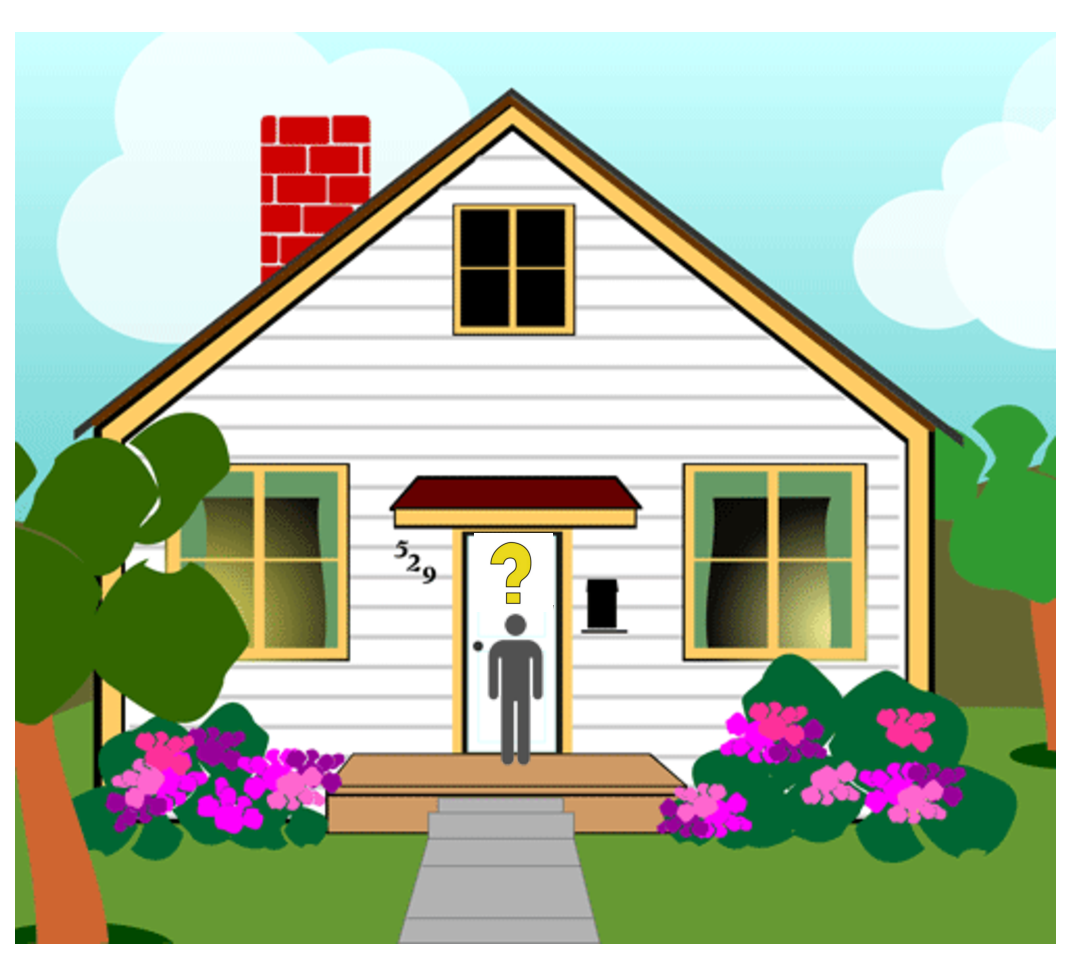
\includegraphics[width=0.35\textwidth]{adlfigs/occupied.pdf}
%\caption{Home Occupancy Example. \label{fig_occupiedexample}}
%\end{figure}
A great deal of research has been done to track the activities of people 
to infer the home occupancy. 
Researchers have made efforts to collect data by sensors, smart phones, 
the calendar, and weather information. 
Most of the approaches that model and predict occupancy primarily use sensor data to detect conditions 
such as room occupancy, use of electrical appliances, water usage, etc.
Several supervised learning approaches, such as kNN, neural networks, rule-based models, 
and Markov chain models have been used to model and predict building occupancy 
\cite{scott2011preheat,alrazgan2011learning,mahmoud2013behavioural,erickson2010occupancy,beltran2014optimal}.  
Using the kNN supervised learning algorithm and monitoring sensor data 
for a portion of the day, 
Scott et al. predict an entire day's occupancy in~\cite{scott2011preheat}. 
A neural network approach using a binary time series based on 
occupancy/unoccupancy along with exogenous input network (NARX) is 
proposed in \cite{mahmoud2013behavioural}. 
Mahmoud et al. tackle the problem by presenting a non-linear autoregressive 
model with an exogenous input (NARX) network. 
Several Markov chain models, like the blended Markov chain, 
closest distance Markov chain, 
and moving-window Markov chains are presented in \cite{erickson2010occupancy}. 
A mixture of multi-lag Markov chains was used to predict the occupancy of 
single-person offices \cite{manna2013learning}. 
In that work, the authors also compare their model with the Input Output Hidden Markov Model, 
First Order Markov Chain and the NARX neural network. 

A recent survey~\cite{kleiminger2014predicting} compares major occupancy 
predictions algorithms against the LDCC dataset~\cite{kiukkonen2010towards}, which was collected by 
GPS and other sensors. 
It shows that time-based presence probability~\cite{krumm2011learning} performs slightly better than the preheat kNN approach~\cite{scott2011preheat}. 
Since the preheat kNN approach~\cite{scott2011preheat} is more widely applicable,  
in that it can be used against both GPS and sensor datasets, 
we set it as a baseline method for comparison. 

%%%%%comment several paragraphs
\iffalse
These superseded learning approaches are classified into several categories. 
The first is on the probability density distribution of key events. 
\cite{tominaga2012unified} proposes that at a time,  a person goes out has a Bernoulli distribution. 
The second effective benchmark approach is kNN. 
kNN approach is employed in 
\cite{scott2011preheat} to predict the occupancy of the left day 
after knowing the occupancy in the partial day. 
It splits the whole day's time into 96 15-minutes intervals 
then to find the top-5 similar day in the training date. 
The average of these similarity is the predictive occupancy. 
The third is the pattern discovery by rule and neural network. 
A rule-based approach is proposed by
\cite{alrazgan2011learning}  for occupancy prediction under the frame work of Decision Guidance Query Language (DGQL). 
A variant of neural network has been proposed by 
\cite{mahmoud2010occupancy}. \cite{mahmoud2010occupancy} converts the data into binary occupancy/unoccupancy data in the first step. Then a model name non-linear autoregressive network with exogenous input (NARX) network is modeled for prediction. 
\cite{mahmoud2013behavioural} also uses binary time series with NARX network. 
The last are models related to Markov chains. 
Several Markov Chains have been compared in the paper of \cite{erickson2014occupancy}, including blended Markov Chain, closest distance Markov Chain, and the moving window Markov Chain with respect to modeling occupancy. 
\cite{erickson2010occupancy} uses moving-window markov chain for occupancy prediction. 
\cite{erickson2013poem} utilizes the markov chain model and blend markov chain model for prediction. 
\cite{beltran2014optimal} uses a blend-markov chain model for prediction. 
\cite{manna2013learning} uses mixture of multi-lag markov chains to predict the occupancy in single person offices. It compares with other previous approaches Input Output Hidden Markov Model, First order Markov Chain and NARX Neural Network. 

This paper contributes the follows:
1) formulate the problem as a temporal mining problem;
2) mine the activity patterns according to time and gap;
3) the occupancy prediction performance of this temporal mining approach works better than kNN for most cases.
\fi

\section{Problem Formulation}
Given $M$ time series, 
each time series $X^{(m)}=X^{(m)}_1, ..., X^{(m)}_t, ..., X_T^{(m)}$ 
represents a sequence of room occupancy of person $m$ inside 
a home over $K$ days, 
where $X_t\in s$ denotes that $X$ belongs to a finite room set $s$ at the sequence number of $t$, 
and $m\in\{1,...,M\}$. 
%Each $X$ is has a start time $X.start$ and an end time $X.end$.  
Let $Z$ denote that the home is unoccupied and $Z\in s$.  %$Z=0$ if a house is unoccupied; $Z=1$ if the house is occupied.  
%Its meaning equals to certain symbols from set $s$. 
We predict whether person $m$ stays at home the rest of a day from time $T$,  i.e. during $T+1$, $T+2$, ..., $\Delta T$, 
 
\begin{equation}
\hat{Y}^{(m)}=\hat{Y}_{T+1}^{(m)},...,\hat{Y}^{(m)}_{T+\Delta T}
\end{equation}
where $Y_{T+\Delta t }^{(m)}=Z$ if person $m$ does not stay at home at time $T+\Delta t $;
otherwise, $Y_{T+\Delta t}^{(m)} \neq Z$. 
%The un-occupancy of the whole house is the intersection of un-occupancy of all people. 
If any person $m$ stays at home $Y_{T+\Delta t}^{(m)} \neq Z$, then this house is occupied $Y_{T+ \Delta t} \neq Z$. 


\iffalse
Given $M$ time series, 
each time series $X^{(m)}=X^{(m)}_1, ..., X^{(m)}_t, ..., X_T^{(m)}$ 
represents a sequence of room occupancy of person $m$ inside 
a home over $K$ days, 
where $X_t\in s$ denotes that $X$ belongs to a finite room set $s$ at the sequence number of $t$. 
Each $X$ is has a start time $X.start$ and an end time $X.end$.  
Let $Z$ denote that the home is unoccupied. 
It equals to certain symbols from set $s$. 
Also, given a time gap from current time $\Delta t$, 
predict whether $Z$ appears at time  $T+\Delta t$

 formulate the occupancy prediction problem as one of 
episode mining and event type time prediction problem. 
\textit{Problem Statement} Given a sequence of the room occupation 
events stream \textit{s} with finite events symbols $\varepsilon$, 
and the target un-occupancy event \textit{Z}, can we
find the frequent patterns $\{\alpha_1,...\alpha_n\}$ 
and can the corresponding episode generative HMM 
$\{\Lambda_{\alpha_1}, ..., \Lambda_{\alpha_n}\}$, 
predict when 
the person leaves $Z.{start}$, 
and when the person comes back $Z.{end}$.?

The training phase is to mine the frequent episodes and connect it with HMM model
as described in \cite{laxman2008stream}. We modify the constraints during episode mining
and keeps the connections between the frequent episodes and HMM the same. 
The training algorithm describes in Algorithm \ref{alg1}.
\fi

%% algorithm 01
\renewcommand{\algorithmicrequire}{\textbf{Input:}}
\renewcommand{\algorithmicensure}{\textbf{Output:}}

\begin{algorithm}
\caption{Trainng Algorithm}
\label{alg1}
\begin{algorithmic} [1]
\REQUIRE training events stream, $S_t=<\hat{E_1}, ..., \hat{E_n}>$; 
target event type Z; size of symbols $\varepsilon$ M; 
window size  \textit{W} preceding the target event Z
\ENSURE Generative model, $\Lambda_Z$ 

\COMMENT{re-organize data}\\
\STATE split data into each day
\STATE rename the symbol based on 15-minutes chuck
\STATE Initialize the partial stream $D_Z= \phi$ before $Z$

\FOR{the data of each day}
\IF{$\exists$ t that $\hat{E_t}=Z$}
\STATE add $S_t=<\hat{E_{t-W}}, ..., \hat{E_{t-1}}>$ to $D_Z$
\ENDIF
\ENDFOR

\COMMENT{build mixture episode generative HMM model}
\FOR{$1<w<W$}
\STATE mine the frequent episodes $\{\alpha_1, ..., \alpha_J\}$ 
\ENDFOR

\STATE connect each episode $\alpha_j $ with a HMM model EGH $\Lambda_{\alpha_j}$ 

\STATE generate episode generative HMM (EGH) mixture model $F(\Lambda)= \sum_1^J \theta_j\Lambda_{\alpha_j}$, where $1 \leq j \leq J$  
with EM algorithm

\STATE Output $\Lambda_Z=\{  (\Lambda_{\alpha_j}, \theta_j ) , j=1,...,J \}$

\end{algorithmic}
\end{algorithm}
\iffalse
From line 1-2, the symbols are reorganized according to the 15-minutes chuck of each day. 
If there are more than one symbols in a 15-minutes chuck, 
the symbol with longest duration event will be chosen. 
This step is to emphasize there is only one place a person stays in the room. 
From line 4-7, the W length sequence before the target symbol Z firstly appears is chosen 
for each day. 
From line 9-11, the frequent episodes are mined. 
From line 12-14, for each episode, a HMM model named EGH is generated and connected. Then a mixture model 
with all these EGHs are calculated with EM algorithm. 

The event time prediction algorithm Algorithm \ref{alg2} is composed of two stages. 
In the first stage from line 1-15,
we could predict whether the next event $E_{t+q}$ is the target event Z or not. 
For each $t$ is greater than W, intercept the sequence of length $W$ 
$X=<E_{t-W}, ..., E_t>$ in line 2. 
If Z is inside the X, then calculate the possible largest Z index $t_{max}$ inside X. 
In lines 4-6 the mixture model is calculated whether the next time $t+1$ would be the target event or not.
In line 8, all the frequent episodes will be checked whether it is inside the sequence X after $t_{max}$
If there is any frequent episode inside X, 
then we could predict the next event $E_{t+1}=Z$. 
That is, if any of the frequent episode happens 
and the value is greater than the threshold, 
then the next event is Z. 

In the second stage, the exact leave and back time prediction of Z is described from line 16-25. 
If a person gets up before sleep, 
generally we don't know when he will leave or come back. 
In this case, the predicted time is based on the average value of the past leave and back time. 
If a person already gets up, 
we mine the episode patterns, 
and predict according to the mixture model. 
This will be detailedly explained in \ref{alg22}.
If a person already leaves, 
the back time prediction is also based on the historical past time with 
a constraint on the leaving time. 
For a person may come back home and stay home for sometimes then go out again, 
we could repeat the second stage until the end of day. 
\fi
%% algorithm 02
\renewcommand{\algorithmicrequire}{\textbf{Input:}}
\renewcommand{\algorithmicensure}{\textbf{Output:}}

\begin{algorithm}
\caption{Prediction Algorithm}
\label{alg2}
\begin{algorithmic} [1]
\REQUIRE Partial day's event stream, $s=<E_1, ..., E_t, ...>$; 
target event type Z; size of symbols $\varepsilon$ M; 
window size  \textit{W} preceding the target event Z;
generative model $\Lambda_Z=\{  (\Lambda_{\alpha_j}, \theta_j ) , j=1,...,J \}$;
threshold $\gamma$

\ENSURE Predict $Z_{leave}$ and $Z_{back}$ if $E_{t+1}=Z$ or $E_{t+1}\neq Z$ 

\FOR{$W \leq t \leq len(s)$}
% get the stream inside a window W
\STATE set $X=<E_{t-W}, ..., E_t>$
\STATE $t_Z=0$

\COMMENT{the probability of X given the mixture model } \\
\IF{$P[X|\Lambda_Z] =\sum_1^J \theta_j\Lambda_{\alpha_j} \geq \gamma$} 

\IF{ $Z \in X$ }
\STATE Set $t_Z$ to largest  t, where $E_{t_{max}}=Z$ and $ t-W \leq t_{max} \leq t$
\ENDIF

\IF{$\exists \alpha \in \{\alpha_1,..., \alpha_J\}$ in X after $t_{max}$}
\STATE Predict $E_{t+1}=Z$
\STATE Record time of each symbol in these frequent episodes \\
%\COMMENT{calculate $\Delta t$ in Algorithm \ref{alg22}}
\ELSE
\STATE Predict $E_{t+1} !=Z$
\ENDIF
\ENDIF %end of the gamma
\ENDFOR

\IF{$E_{t+1} =Z$}

\IF{$t_Z$ happens before a person gets up}
\STATE $S_{leave}= \frac{\sum_1^J Z_{leave}}{J}$ where $Z_{leave}= t_{Z_{first}} \in \alpha_j$
\STATE $S_{back}= \frac{\sum_1^J Z_{back}}{J}$ where $Z_{back}= t_{Z_{last}} \in \alpha_j$
\ELSIF{$t_Z$ happens before a person gets up}
\STATE $S_{leave}$ and $_{back}$ are predicted by mixture models
\ELSE
\STATE $S_{back}= \frac{\sum_1^K Z_{back}}{K}$ where $Z_{leave}= t_{Z_{last}} \in \alpha_j$ 
and $Z_{leave}$ has a noise $\epsilon$

\ENDIF

\ENDIF
\STATE Output $E_{t+1}$, $S_{leave}$, $S_{back}$

\end{algorithmic}
\end{algorithm}





\section{Temporal Mining Mixture Model}
We use a three-pronged approach to tackle the problem of mining and predicting unoccupancy, as 
shown in Figure~\ref{fig_framework}.
\begin{figure}[h]
\centering
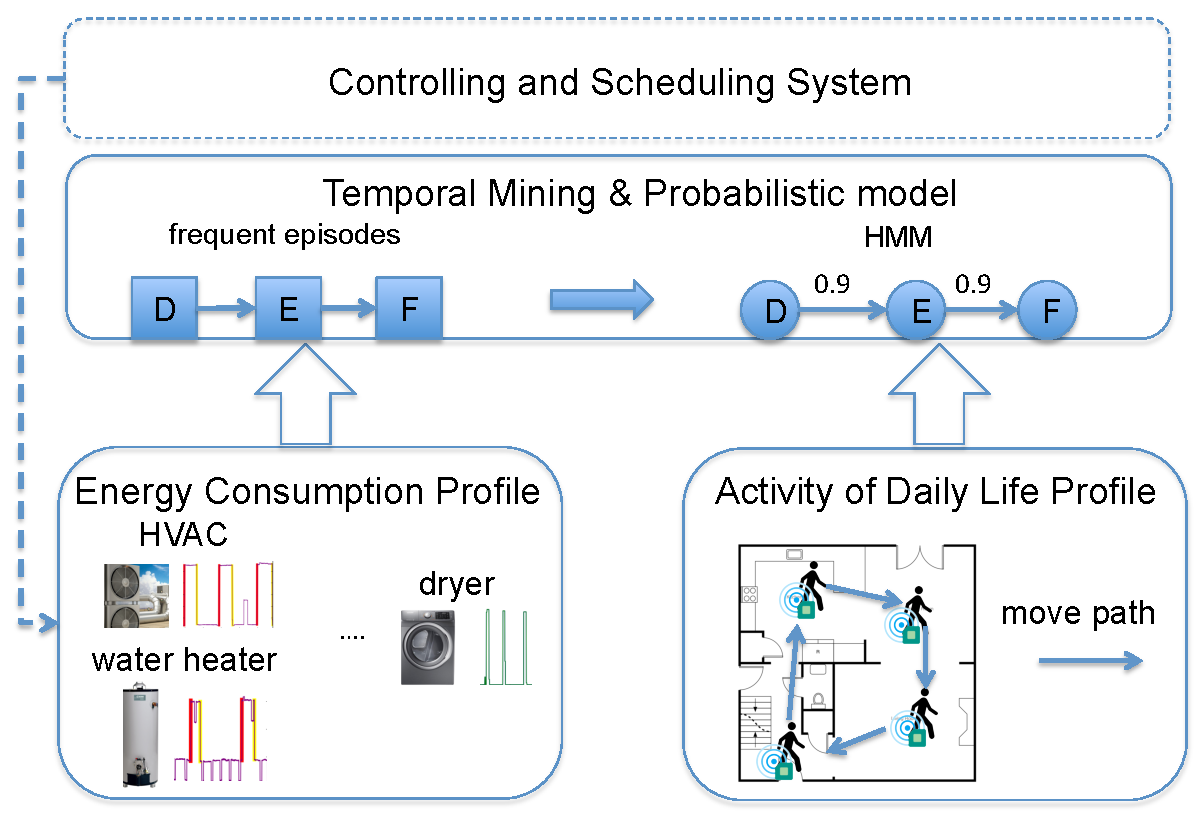
\includegraphics[width=0.5\textwidth]{adlfigs/framework.pdf}
\caption{Occupancy Prediction Framework.\label{fig_framework}}
\end{figure}
Given indoor activities time series of a person over a period of time, 
first, we use an episode mining algorithm to discover frequent episodes from the past days' data. Then we connect each episode with an EGH and build a mixture EGH model. 
Based on the mixture model, we predict when each person will leave and come back the house. 
If all people leave, then the house is unoccupied. 

%Before formalizing the problem statement, we introduce several concepts and notations. 

\textit{Episode} 
An episode is a collection of ordered events. 
Here an episode refers to an ordered events which are 
highly relevant to the occupancy status inside a building. 
For instance, we represent 'S' as sleep, 
'K' as kitchen, and 'Z' as going out. 
If an episode $S \rightarrow K \rightarrow Z$ is found, 
the story is described as a person getting up, 
going to the kitchen for breakfast, and then leaving the house. 
An episode $\alpha$ is composed 
of a series of ordered events
$\alpha=\langle X_1,..,X_t,...X_T \rangle$, 
where $X_t$ denotes that $X$ occurs at a sequence of $t$.  
The event $X_t$ may be the point event or dwelling event. 
The dwelling event
has a start time $X.start$ and end time $X.end$. 
In this paper  $X$ denotes a dwelling event and 
represents which room a person stays 
inside a building, i.e., this building is \emph{occupied}. 
Since $Z$ denotes a room is unoccupied, 
$Z.start$ is the point at which a person or all people inside the building leave, and 
$Z.end$ is the point at which a person or all people come back. 

%\textit{EGH} Episode generative HMM model is a 
%type of HMM model which connects each episode $\alpha$ 
%with a special HMM model $\Lambda_\alpha$. 
%The uniqueness of the EGH is that 
%the transition matrix and 
%emission matrix is only decided by a noise parameter $\eta$. 
%The value of $\eta$ is computed based on the frequency of the 
%corresponding episode $\alpha$. 

\subsection{Time-gap Constraint Episode Mining}
\textbf{Episode Mining}
Episode mining has been studied in previous research \cite{mannila1997discovery}. 
It uses a non-overlap mining approach to find the frequent episodes. 
Episode mining has been applied to energy disaggregation to help conserve energy in buildings~\cite{shao2013temporal} in sustainability research. 
In contrast with previous research, 
the events in this application of occupancy prediction 
dwell at an event for a period of time. 
As a result, we extend the above two 
episode mining algorithms~\cite{laxman2008stream,patnaik2008inferring} 
and enforce more constraints.
One change is to 
adopt right alignment for the first element in the episode mining. 
%In the example of $AB$, 
%the mined second instances is $\langle A_9,B_{11} \rangle$. 
The second modification is to 
add time constraints and 
apply gap duration constraints between 
two consecutive events inside an episode. 
%Figure \ref{fig_durationgapconstraint} shows an example of time-gap constraint episode. 
%\begin{figure}[h]
\centering
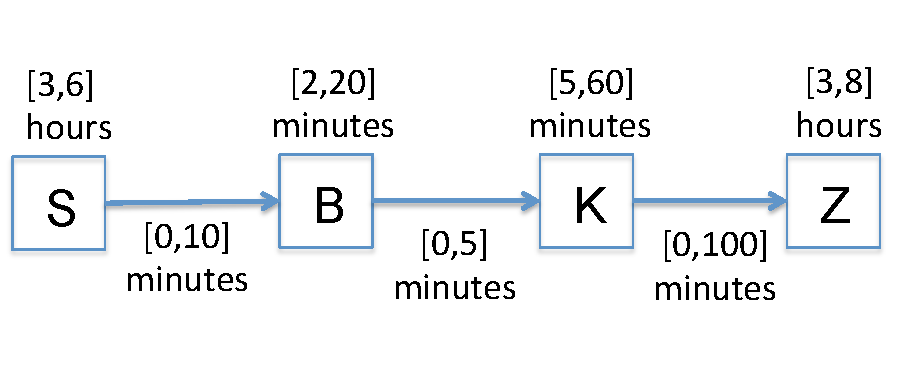
\includegraphics[width=0.5\textwidth]{adlfigs/durationgapconstraint.pdf}
\caption{Example of Duration-gap Constraint Episode.\label{fig_durationgapconstraint}}
\end{figure}

\begin{figure}[!hbtp]
\centering
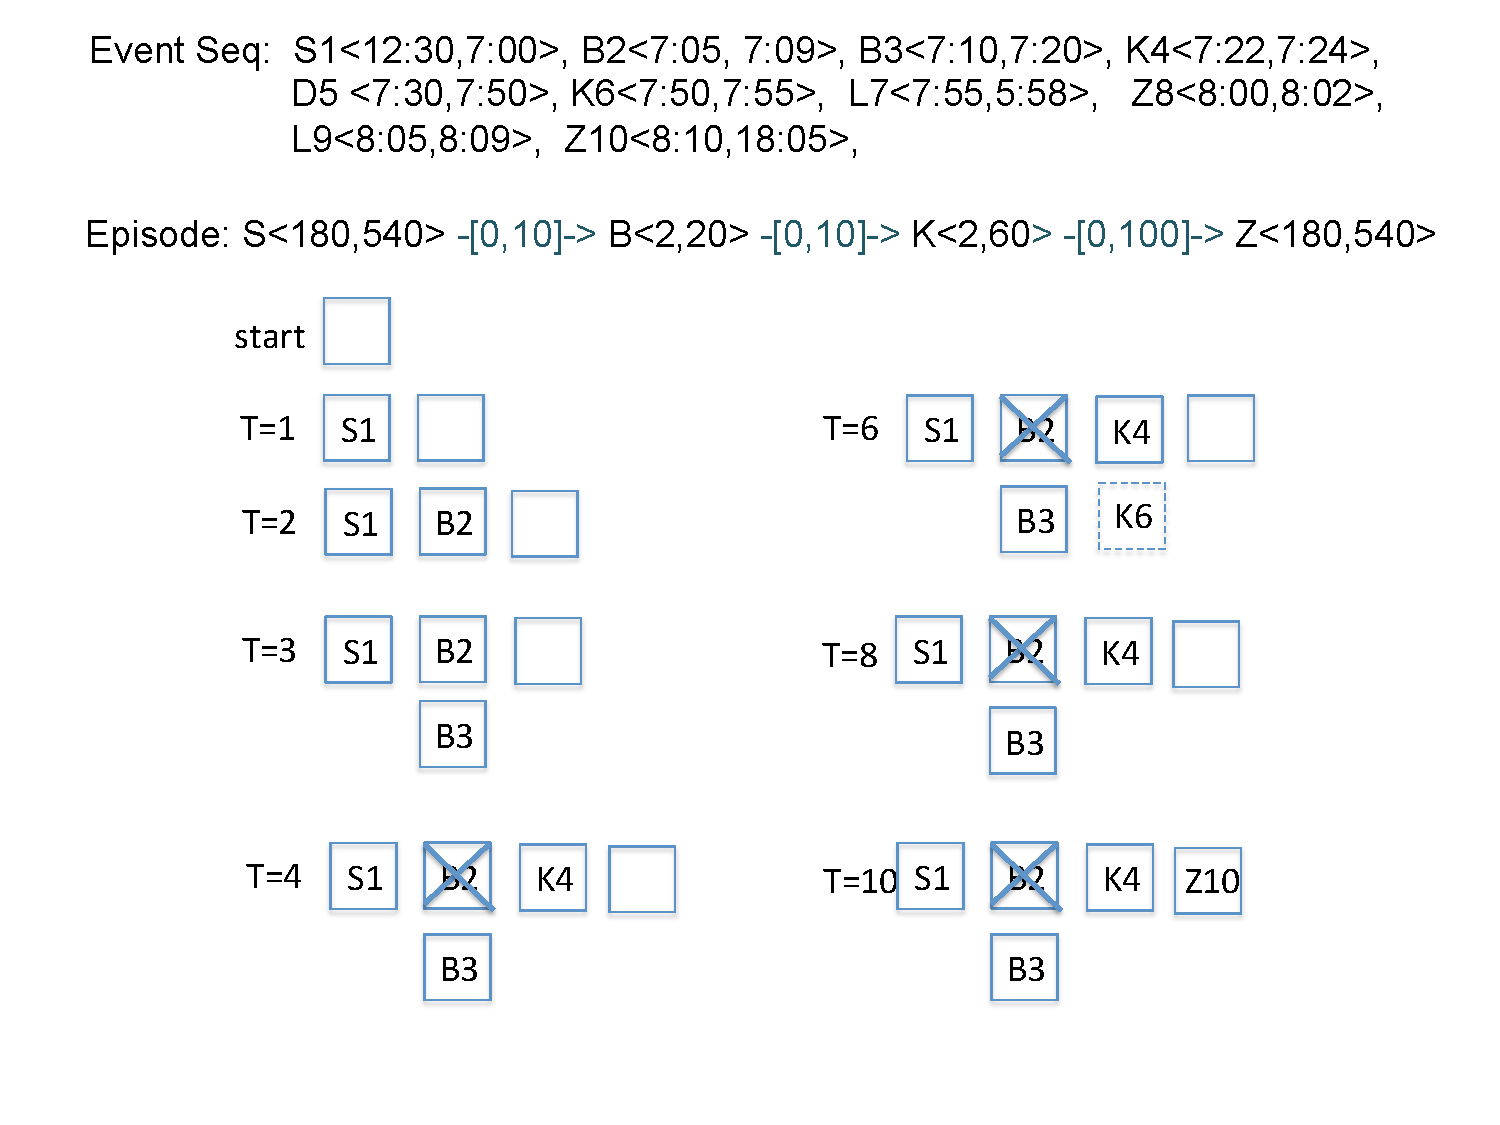
\includegraphics[width=0.5\textwidth]{adlfigs/MingExample.pdf}
\caption{Time-gap constraint episode mining example.\label{fig_MingExample}}
\end{figure}

Figure~\ref{fig_MingExample} shows a time-gap constraint episode mining example. 
Let us assume we have a frequent episode $S\rightarrow B \rightarrow K\rightarrow Z$. 
We then add the time constraints to each event $\{S,B,K,Z\}$. 
The dwelling duration of $S$ is 3 to 6 hours,   
of $B$ is 2 to 20 minutes, 
of $K$ is 5 to 60 minutes, 
and of $Z$ is 3-9 hours. 
In addition, we set gap duration between any two consecutive events. 
The gap duration of $SB$ is calculated as $\Delta{SB} = B.start-S.end$. 
We set the maximal gap time between SB, BK, and KZ as 
10 minutes, 40 minutes and 100 minutes; 
the minimal gap time is 0. 
Then we have a stream composed of the sequence of dwelling events "Event seq," as shown 
in Figure~\ref{fig_MingExample}.  
 The time-gap constraint episode mining process 
 to discover a frequent episode uses the following method. 
 Let the $node$ structure denotes each element in any episode,  
as depicted as a square box in Figure~\ref{fig_MingExample}.  
Let $waits$ refer to a structure which pairs with an episode 
and has the same length of this episode. 
Initially, a $waits$ structure related to episode $S\rightarrow B \rightarrow K\rightarrow Z$ is created. 
A $node$ structure related to $S$ is created 
and it waits for the first 
element of the episode $S\langle 180, 360 \rangle $. 
When $T=1$, the duration of $S_1$ is checked. 
Since $S_1$ is in the range of $3-6$ hours, 
$S_1$ passes and is put into the node structure $node$ related to $S$. 
Next a new $node$ structure is created to wait for $B\langle 2, 20 \rangle $. 
When $T=2$ and $T=3$, both $B_2$ and $B_3$ 
are qualified in terms of the time constraints and 
the gap constraints; 
e.g., the gap between $S$ and $B$ $\Delta SB$ should 
be between 0 and 10 minutes. 
These two nodes $B_2$ and $B_3$ are then input into the 
$waits$ structure. 
At the same time, 
a new $node$ structure is created for $K\langle 5, 60 \rangle $. 
When $T=4$, the gap between $\langle B_3, K_4 \rangle$ 
is satisfied with the distance condition between 
$B$ and $K$ 0-40 minutes. 
However, the gap between $\langle B_2, K_4 \rangle$ 
is longer than the constraint gap. 
Therefore, $B_2$ is canceled out. 
Now a new $Z$ waits for the symbol $Z\langle 180, 540 \rangle$. 
When $T=6$, the gap from $B_2$ to $K_6$ is 
too large. Therefore, $K_6$ is not added into the $node$ $K$ structure in $waits$.
When $T=8$, the duration of $Z_8$ does not qualify for the condition of between 3-9 hours,  
so $Z_8$ is not added. 
When $T=10$, the duration of $Z_{10}$ meets the requirement of between 3-9 hours 
and its distance to $K4$ meet the requirement 
of $\Delta KZ \in [0,100]$ minutes. 
Thus $Z_{10}$ is added into the $node$ $Z$ structure in $waits$.
Therefore, complete mining of an episode is complete, and 
we have mined two instances here; $S_1B_3K_4Z_{10}$ and $S_1B_3K_6Z_{10}$. 

%This complete gap-constraint episode mining on dwelling events 
%is described in detail in Algorithm \ref{alg_episodeMiningConstraint}
%\ref{alg_episodeMiningConstraint_2e} 
%in the appendix section.

%Non-overlap episode mining is defined as \textit{Definition}. 
\subsection{Mixture EGH}
\textbf{Episode Generating HMM}
Episode generative HMM (EGH) model is a 
type of HMM model which connects with frequent episode, 
and the more frequent an episode inside a sequence, 
the likelihood of the state sequence including this episode is larger~\cite{laxman2008stream}.  
%$\alpha$ with a special HMM model $\Lambda_\alpha$. 
The uniqueness of the EGH is that 
the transition matrix and 
emission matrix is only decided by a noise parameter $\eta$. 
The noise parameter $\eta$ of frequent episode $\alpha$ 
is calculated as $\eta=\frac{T-Nf_{\alpha}}{T}$,  
where $T$ is the training data stream length, 
$\alpha$ is the frequent episode, 
$N$ is the length of frequent episode $\alpha$, 
$f_{\alpha}$ is the frequency over the time $T$.

%% not sure whether should be included 09112015
In the mixture EGH model shown in Figure \ref{fig_egh}, 
the transition matrix of an EGH is given as an example. 
Let us assume we have a N-node frequent episode $S\rightarrow B\rightarrow Z$, where $N=3$.
We define 2N number of hidden states; 
N for episode states, and N for noise states. 
The noise states are $\{W, X, Y\}$. 
An episode state transfers to another episode state 
at the probability of $1-\eta$.
An episode state transfers to a noise state 
at a probability of $\eta$. 
A noise state transfers to another noise state 
at a probability of $1-\eta$. 
To calculate the emission matrix, first we 
let M denote the total number of symbols in the event stream. 
For any hidden states in the episode, M has a delta function emission. 
Whenever it is visited (right alignment of the first element in the episode, 
left alignment for the left elements in the episode), 
it will generate the same observation symbol. 
For any noise hidden states, it emits any of the symbols from the $M$ 
observation symbols with a uniform distribution at probability $\frac{1}{M}$. 
\begin{figure}[!hbtp]
\centering
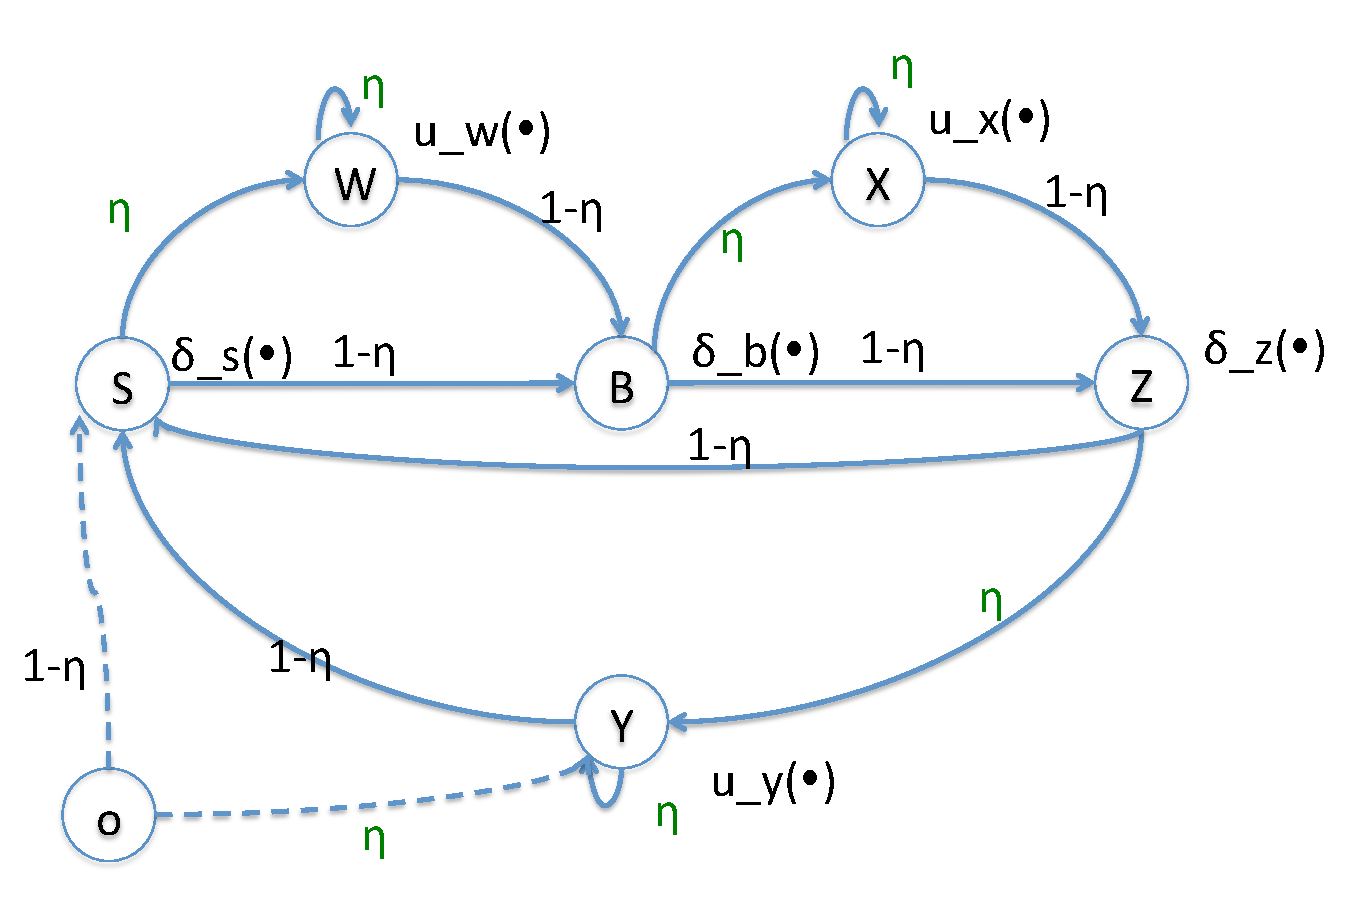
\includegraphics[width=0.5\textwidth]{adlfigs/egh.pdf}
\caption{States Transition of Episode Generating HMM (EGH).\label{fig_egh}}
\end{figure}


Theorem \ref{theorem1} from \cite{laxman2008stream} is crucial.  
The theorems in \cite{laxman2008stream}
prove that the more frequent an episode is inside a sequence, 
the greater the likelihood of the state sequence including this episode. 
The proof for this theorem is explained in detail in \cite{laxman2008stream}. 


\newtheorem{mydef}{THEOREM}
\begin{mydef}
\label{theorem1}~\cite{laxman2008stream} 
Let $D_Z={X_1,..., X_K}$ is the given sequence data,  $\varepsilon$ is the symbol set, 
and the size of these symbols is $M$. 
Given two frequent N-node episodes $\alpha$ and $\beta$ with frequency $f_{\alpha}$ 
and $f_{\beta}$. Their corresponding EGH is $\Lambda_{\alpha}$ and $\Lambda_{\beta}$. 
The most likely state sequence for episode $\alpha$ and $\beta$ are
$q_{\alpha}^*$ and $q_{\beta}^*$. 
The noise parameters of these two EGH are 
$\eta_{\alpha}$ and $\eta_{\beta}$. 
Assume both of these noise parameters are less than $\frac{M}{M+1}$, 
we have 
(1) if $f_{\alpha} > f_{\beta}$, then $P(D_Z, q_{\alpha}^*| \Lambda) > P(D_Z, q_{\beta}^*| \Lambda)  $
(2) if $P(D_Z, q_{\alpha}^*| \Lambda) > P(D_Z, q_{\beta}^*| \Lambda)  $, $f_{\alpha} > f_{\beta}$
\end{mydef}

\textbf{Mixture Model}
The mixture EGH model is fully discussed in previous work \cite{laxman2008stream}.
This model 
gives different weights to each EGH
to predict a target event. 
We can assume we obtain whether an episode occurs on a certain day. 
Let $D_Z=\{X_1,..., X_K\}$ denote the $K$ days data set. 
$F=\{\alpha_1, ... \alpha_J\}$ denote the frequent episodes in the dataset $D_Z$. 
An EGH $\Lambda_{\alpha_j}$ 
is associated with frequent episode $\alpha_j$.
$\Lambda_Z$ denotes a mixture EGH model. 
The likelihood of $D_Z$ under the mixture model is written as Equation (\ref{eq_mixture}).
\begin{eqnarray}
\label{eq_mixture}
Pr(\Lambda|Z) &=& \prod_{i=1}^K P[X_i|\Lambda_Z] \\
			&=& \prod_{i=1}^K ( \sum_{j=1}^J \theta_j P[X_i| \Lambda_{\alpha_j}])
\end{eqnarray}
where $\theta_j$ is the mixture coefficient of $\Lambda_{\alpha_j}$ and it subjects to 
$\sum_{j=0}^J \theta_j=1$ 

The parts inside Equation (\ref{eq_mixture}) are additive; 
the coefficients $\theta$ are computed by EM algorithm. 
%The detailed description is algorithm %%%\ref{alg3} 
%in the appendix section.
%% algorithm 03
\renewcommand{\algorithmicrequire}{\textbf{Input:}}
\renewcommand{\algorithmicensure}{\textbf{Output:}}

\begin{algorithm}
\caption{EM Algorithm for mixture EGH}
\label{alg3}
\begin{algorithmic} [1]
\REQUIRE day episode matrix, 
each element $e_{ij}$ records for each day whether an episode $j$ happens in day $i$;
frequent episodes $F=\{\alpha_1, ..., \alpha_J\}$;
symbol set $\varepsilon$;
threshold $\gamma$

\ENSURE the parameters for mixture EGH $\Lambda_Z=\{  (\Lambda_{\alpha_j}, \theta_j ) , j=1,...,J \}$


\STATE calculate the number of episodes J, and number of days K
\STATE calculate all $\eta$s' threshold value $mThreshold= \frac{M}{M+1}$

\COMMENT{initialize all the thetas to be $\frac{1}{J}$}
\COMMENT{calculate the total frequency for each episode over training time series}
\COMMENT{ calculate the $eta$ value}
\FOR{$0 \leq j \leq J$}
\STATE $\theta[j]= 1/J$
\STATE $episodeFreq[j] = \sum_i^K e_{ij}$
\ENDFOR

\STATE select those frequent episodes starting with 'S' and ending with 'Z' and separate these 
episodes by workday or holiday

\COMMENT {calculate $eta$ for each episode} 
\FOR{$0 \leq j \leq J$}
\STATE $\eta[j]= 1-episodeLen[j]*episodeLen/T$
\ENDFOR

\COMMENT{likelihood prediction of each episode $j$ in the $k$th day}

\FOR{$0 \leq i \leq K$}
\FOR{$0 \leq j \leq J$}
\STATE $likelihood_{ij} = \frac{1-\eta[j]}{\eta[j]/M} ^ {episodeLen[j]*e_{ij}}$
\ENDFOR
\ENDFOR

\COMMENT{calculate the obj value based on J, K, $likelihood_{ij}$ and $\theta$}
\WHILE{$newObj- obj > \gamma$}
\STATE $\theta_{new}=[]$
\FOR{$0 \le l \le J$}
\STATE $temp=0$
\FOR{$0 \le j \le K$}
%\COMMENT{calcuate the new likelihood with Bayes rules}
\STATE $temp = temp+ \frac{\theta_l*likelihood_{il}}{ \sum_0^J { \theta_j*likelihood_{ij}}}$

\ENDFOR
\STATE $\theta_{new}[l] = temp/K $
\ENDFOR

\STATE calculate the newObj
\IF{$newObj-obj > \gamma$}
\STATE $obj=newObj$
\STATE $\theta_{new} = \theta$
\ENDIF

\ENDWHILE

\STATE Output $\Lambda_Z=\{  (\Lambda_{\alpha_j}, \theta_j ) , j=1,...,J \}$

\end{algorithmic}
\end{algorithm}
During the initialization %line 1-10
part of the EM algorithm, 
the episode frequency over the times series T over $K$ days is calculated. 
Specific frequent episodes ended with target event 'Z' are selected. 
Optionally, 
we could add special constraints on episodes, starting with 
certain event type 'S'. 
%calculated in lines 11-16. 
% not sure this paragraph to be added or not
In the expectation step, 
one key part is the likelihood value of each episode $\alpha_j$ in time series $X_i$.
The likelihood value is computed as Equation (\ref{eq_likelihood});
Then Bayes rules is applied to compute the new coefficient $\theta_{new}$. 
\begin{equation}
\label{eq_likelihood}
Pr(X_i| \Lambda_{\alpha_j}) = (\frac{\eta_{\alpha_j}}{M})^{|X_i|} (\frac{1-\eta_{\alpha_j}}{\eta_{\alpha_j}/M})^{|\alpha_j|f_{\alpha_j}(X_i)}
\end{equation}
In the maximization step, 
we update the objective value based on Equation (\ref{eq_mixture}) until it converges, i.e., 
until the difference of two consecutive objective values 
is smaller than a threshold.%$\gamma$.


\subsection{Predict When the Target Event Occurs}
Target event prediction is studied in~\cite{laxman2008stream},  
but only insofar as it predicts whether a target event will occur, 
rather than when the target event will happen. 
Our occupancy prediction algorithm enriches the previous 
event prediction algorithm by breaking into three sub-problems; whether the target event un-occupancy $Z$ will appear, when the target event $Z$ starts, and when the target event $Z$ ends. 

Since the solution to the first sub-problem is similar to 
previous work, 
this sub-section emphasizes on the last two sub-problems. 
After obtaining the result of the first sub-problems, 
we assume we already know that the target event $Z$ will surely happen, 
and so we need to predict when the person leaves or comes back. 
The leaving time corresponds to the start time of dwelling event $Z.start$ and 
the returning time refers to the end time of dwelling event $Z.end$. 
%This prediction algorithm is described in algorithm \ref{alg22}. 

After running episode mining and mixing the EGH model, 
we have obtained all the frequent episodes $F=\langle \alpha_1,..., \alpha_J \rangle$, 
the corresponding EGH $\Lambda_{\alpha_j}, j=1...J$ with noise parameter $\eta_j$, 
and the mixture models $\Lambda_Z$ with coefficients $\theta_j$.
We use the coefficient of these mixture models to predict the leave time and return time of 
target event $Z$. 
 Each day is cut into three phases: 1) Before a person gets up; 
2) After the person gets up but before the person goes out;
and 3) After the person goes out but before they come back. 
\begin{enumerate}
\item
Usually before a person gets up, there is only one frequent episode named 'SZ'. 
The start time and end time of $Z$ depends on 'S'. 
Therefore $Z.start$ and $Z.end$  are calculated by the probability density function of 
going out and coming back time in the past days. 
\item
After the person gets up, if he/she has a lot of activities at home, 
there are several frequent episodes that are mined before the person leaves home. 
If there are several frequent episodes ending with $Z$,  
the leave time and return time of each episode is checked to determine
whether they are in a range of probability density function (PDF) value in the past. 
If yes, the mean value of these episodes are recorded. 
Since each episode generates an EGH, 
the mixture EGH model computes a weight for each EGH as coefficients. 
The leave time $Z.start$ and back time $Z.back$ are 
the weighted mean leave time and back time of these frequent episodes. 
\item
After a person leaves home, 
we already know when the person leaves home $Z.start$. 
If the person has come back, 
nothing needs to be predicted. 
If the person has not come back,  
the return time $Z.end$ is the weighted 
 historical return time of mined 
frequent episodes, 
viz. the probability density function of backing time based on the 
time-constraint going out time.
\end{enumerate}

\iffalse
The algorithm \ref{alg22} 
uses partial day of test data $s$, 
all the frequent episodes  $epis$, 
the frequent episodes $F$ in partial day of $s$, 
the mixture model $\Lambda_Z$, 
to predict when the person leaves or comes back home. 
The partial day is cut by partial index $pIndex$. 
Each day is cut into three phases, before the person gets up; 
after the person gets up but before the person leaves home;
after the person comes back home. 

In the first two phases, before the person leaves, 
the PDF leave time and back time are calculated from line 2-4. 
Usually before a person gets up, there is only one frequent episode named 'SZ'. 
After the person gets up, he/she has a lot of activities at home, 
there are several frequent episodes mined before the person leaves home. 
In case there are several frequent episodes in lines 6-12, 
the leave time and back time of each episode is checked
whether they are in a range of PDF value in the past. 
If yes, the mean value of these episodes are recorded from line 14-17. 
If there are several frequent episodes with corresponding EGH, 
the leave time $Z_{leave}$ and back time $Z_{back}$ is the weighted 
mean leave time and back time of each episode in lines 18-21. 

In the third phase, after the person leaves home, 
we already know when the person leaves home $Z_{leave}$ 
but needs to predict when the person comes back $Z_{back}$. 
If the person has come back, that means $Z_{back}$ is not equal to $Z_{leave}$. 
We don't need to do anything. 
If the person has not come back, that means $Z_{back}$ equals to $Z_{leave}$. 
The back time is the past weighted back time from line 28-34. 
%% algorithm 22, an extention of algorithm 2
\renewcommand{\algorithmicrequire}{\textbf{Input:}}
\renewcommand{\algorithmicensure}{\textbf{Output:}}

\begin{algorithm}
\caption{ Target Event Occurs Time Prediction Algorithm}
\label{alg22}
\begin{algorithmic} [1]
\REQUIRE 
partial day cut point $pIndex$, $s[1:pIndex]$ is known,  and $s[pIndex:96]$ for prediction;
partial day event stream $s=\langle E_1,..., E_{pIndex} \rangle$;
all the episodes $epis$, $\forall E \in \alpha$ and $\forall \alpha \in epis$, E has $E.{start}$ 
and $E.{end}$; 
frequent episodes $F=\langle \alpha_1,..., \alpha_J \rangle$ inside $s[1:pIndex]$;
EGH model $\Lambda_{\alpha_j}$ with noise parameter $\eta_j$ where $j=1...J$
EGH mixture model coefficients $\Theta=\langle \theta_1,...,\theta_J \rangle$;
the slot number noise parameter $\epsilon$  ; 
target event $Z$
\ENSURE Predict target event leaving time $Z_{leave}$ and back time $Z_{back}$
 
\IF{$Z  \notin s $}%\COMMENT{predict before the person leaves home}
\STATE choose episodes $\alpha.ev={'SZ'}$ 
\STATE $Z_{leave} = \frac{\sum_1^K Z.start}{|\alpha|} $
\STATE $Z_{back} = \frac{\sum_1^K  Z.end}{|\alpha|}  $
\IF{$len(F)>1$}%\COMMENT{if there are several episodes to predict 'Z'}
\FOR{$\alpha_j \langle e_1,..., e_j \rangle \in F$}
%\IF{$\alpha_j.ev='SZ'$} % 'SZ' has been calculated,no need to calculate again
%\STATE break
%\ENDIF
\IF{$pIndex \in ( \alpha_j. ev[-2].start - \epsilon, \alpha_j.ev[-2].start+ \epsilon )$}
\STATE $leaveMap[\alpha_j.ev]=\alpha_j.leave$
\ENDIF
\IF{$pIndex \in ( \alpha_j. ev[-2].end - \epsilon, \alpha_j.ev[-2].end+ \epsilon )$}
\STATE $backMap[\alpha_j.ev]=\alpha_j.back$
\ENDIF 
\ENDFOR
\IF{$len(leavingMap) !=0 $} % for the average
\STATE $leaveSlotMap[\alpha_j.ev] =\frac{\sum_1^K leavingMap.get(k)}{K}$
\STATE $backSlotMap[\alpha_j.ev] = \frac{\sum_1^K backMap.get(k)}{K}$
\ENDIF % this is for the len\\
\IF{$K=len(leaveSlotMap)>1$}%\COMMENT{There are other frequent episodes except 'SZ'}
\STATE $Z_{leave}= \frac { \sum_{k=1}^K leaveSlotMap.get(k) * \theta_k } {K}$
\STATE $Z_{back}= \frac { \sum_{k=1}^K backSlotMap.get(k) * \theta_k } {K}$
\ENDIF
\ENDIF %this is for len(F)>1 
\ENDIF %this is for if Z \notin S \\
\IF{$Z  \in s $}%\COMMENT{if the person has left home}
\STATE $Z_{leave}=s.firstindex[Z]$ % the position where $Z$ first appears
\STATE $Z_{back}=s.lastindex[Z]$ % the position when $Z$ lastly appears\\
%\STATE backSlotMap=\{\}
\IF{$Z_{leave}=Z_{back}$} %\COMMENT{The person hasn't come back}% the person hasn't come back
% get the average of those time
\FOR{$\alpha_j \langle e_1,..., e_j \rangle \in F$}
\IF{$Z_{leave} \in [\alpha_j.ev[-2].end - \epsilon, \alpha_j.ev[-2].end + \epsilon ]$}
\STATE $backSlotMap[\alpha_j.ev] = \alpha_j.leave$
\ENDIF
\ENDFOR
\STATE $Z_{back}= \frac { \sum_{k=1}^K backSlotMap.get(k) * \theta_k } {K}$
\ENDIF
\ENDIF
\STATE Output the slot number when the person leaves $Z_{leave}$ and comes back $Z_{back}$
\end{algorithmic}
\end{algorithm}
\fi

 






\section{Experiment Results}
We have conducted experiments on three datasets, where each dataset is obtained by monitoring 24-hour activities of two adults in a house via RFID. 
All these activities occur in twelve rooms; the basement, bathroom, bedroom, dining room, hallway, kitchen, living room, mudroom, nursery, outside-front, outside-back, and upstairs.  
%\begin{table}[h]
%\centering
%\caption{Datasets summary.} 
%\label{tab_dataset}}
%\begin{tabular} {|c|c|c|c|}
%\hline
%Dataset & Number of entries & Period(day) & Start date\\
%\hline
%study10  & 6596 & 12 & 02/10/2014\\
%\hline
%study11  & 1696 & 10 & 01/29/2014\\
%\hline
%study14 & 3453 & 13 & 12/09/2013\\
%\hline
%\end{tabular}
%\end{table}
The dataset comprises events in the form of timestamped room occupancy data points. For instance, an event can correspond to person 1 being in the kitchen at 7:00 am. The summary of these three datasets is shown in Table~\ref{tab_dataset}.
%Study10 spans 12 days from 02/10/2014 to 02/21/2014 and Study11 spans 10 days from 01/29/2014 to 02/07/2014, and Study14 spans 13 days from 12/09/2013 to 12/21/2013.
We define \textit{unoccupancy} of a person as one of these conditions: the person leaves the {\em outside-front} or {\em outside-back} for more than 30 minutes; the person stays in the living room or dining room for more than 9 hours without any other activities; or the gap between any two events is more than 30 minutes. 
Since our research goal is to automate the turning on and off of the HVAC system at least 30 minutes before occupancy, the first and third constraints are in place. We are only interested in events where the {\em unocupancy} period is for an extended duration ($>$ 30 minutes). The second constraint comes from our observation that if a person stays in one room for more than 9 hours without moving to other rooms, 
this usually means that the person has gone out but left the RFID equipment at home. 
Furthermore, we delete events with a duration less than 
2 minutes since these correspond to the individual walking back and forth across rooms and generally do not contribute to meaningful episodes. We conduct four types of experiments to compare four approaches; 
kNN, mixture EGH, PDF, and support vector regression (SVR). 
For each dataset, we use $2/3$ of the data for training and the remaining $1/3$ of the data as a test. 
Following the approach in~\cite{scott2011preheat},
we organize one day's data into 96 15-minute chunks. 
For the test data, we assume that we only know some of the 15-minute chunks. Our target is to predict the occupancy in the rest of the day, or 30 minutes ahead. 

\subsection{Occupancy Prediction of Individuals}
%We apply three approaches, kNN, PDF based and mixture EGH time prediction model. 
%Similar to \cite{scott2011preheat},
%we organize one day's date into 96 15-minutes intervals with mixture EGH model. 
%Then we split the test date into three phases: 
%(1) before getting up, (2) after getting up and before going out, 
%(3) after going out and before coming back. 
%Thus our problem becomes to predict when the person going out 
%and when the person comes back. 
%Corresponding to these four phases, we adopt three different approaches. 
%For stage (1), the probability density function of going out and combing back event is calculated. 
%For stage (2), a duration-constraint episode mining and episode generative HMM is applied. 
%For stage (3), the probability density function of backing time based on 
%the time-constrains going out time is computed. 

%The results are shown in Figure~\ref{fig_study10} and Table~\ref{tab_individualResults}
%Figure~\ref{fig_study11}, and Figure~\ref{fig_study14}. 
%Each of these figures 

\begin{table*}[t]
%\vspace{0.2cm}
\hfill
%\begin{minipage}[t]{1.0\linewidth}%

\caption{Precision Recall F-measure Comparison of Individual and Whole House Occupancy Prediction in Study 14.}
\label{tab_individualResults}
%\tbl{Precision Recall F-measure Comparison of Individual and Whole House Occupancy Prediction in Study 14.\label{tab_individualResults}}{
%\begin{center}
%\makebox[\textwidth]{
\centering
\small
\setlength\tabcolsep{2pt}
\begin{tabular} {|l|l|l|l|l|l|l|l|l|l|l|l|l|l|l|l|}
\hline
\multirow{2}{*}{Dataset}&\multirow{2}{*}{Date}&\multirow{2}{*}{Person} & \multicolumn{3}{|c|}{EGH}&\multicolumn{3}{|c|}{kNN} &\multicolumn{3}{|c|}{SVM}   \\
\cline{4-12}
&&& precision & recall &fmeasure &precision & recall & fmeasure &precision & recall & fmeasure \\
\hline
\multirow{3}{*}{study10}  & 02/17/2014 & person2& \textbf{1.00} & \textbf{1.00}&\textbf{1.00} & 0.99 & 0.98 & 0.98 &0.71 &0.76 & 0.71\\
\cline{2-12}
& 02/19/2014 & person1& 0.98 & 0.99 &0.98&  \textbf{0.99} &  \textbf{0.99} &  \textbf{0.99} & 0.71 & 0.76 & 0.70 \\
\cline{2-12}
& 02/20/2014 & person2&  \textbf{0.93} &  \textbf{0.92} &  \textbf{0.92} & 0.92 & 0.91 & 0.90 & 0.72 & 0.77 & 0.72\\
\cline{2-12}
& 02/20/2014 & person1&  \textbf{0.95}& \textbf{0.94} & \textbf{0.94} & 0.94	& 0.93 & 0.93 & 0.71 & 0.77 & 0.72 \\
\cline{2-12}
& 02/20/2014 & \textbf{wholehouse}&  \textbf{0.92}& \textbf{0.92} & \textbf{0.91} & 0.91	& 0.89 & 0.91 & 0.79 & 0.74 & 0.74 \\
\hline
\hline
\multirow{3}{*}{study11}  & 02/04/2014 & person2& 0.93 & 0.93 & 0.92  & \textbf{0.95} & \textbf{0.95} & \textbf{0.95} & 0.71 & 0.77 &0.72\\
\cline{2-12}
& 02/04/2014 & person1& 0.93 & 0.93 & 0.92  & \textbf{0.95} & \textbf{0.95} & \textbf{0.95} & 0.70 & 0.77 & 0.71  \\
\cline{2-12}
& 02/05/2014 & person2&  \textbf{0.85} &  \textbf{0.92} &  \textbf{0.86} & 0.87 & 0.87 & 0.84 & 0.71 & 0.76 & 0.71 \\
\cline{2-12}
& 02/05/2014 & person1&  \textbf{0.84} &  \textbf{0.90} &  \textbf{0.84} & 0.79 & 0.90 & 0.80  & 0.70 & 0.77 & 0.71   \\
\cline{2-12}
& 02/04/2014 & \textbf{wholehouse}&  \textbf{0.918}& \textbf{0.924} & \textbf{0.913} & 0.916	& 0.921 & 0.911 & 0.77 & 0.69 & 0.71  \\
\cline{2-12}
& 02/05/2014 & \textbf{wholehouse}&  \textbf{0.90}& \textbf{0.84} & \textbf{0.84} & 0.88	& 0.81 & 0.81 & 0.74 & 0.70 & 0.70\\
\hline
\end{tabular}
%}
%\end{center}
%\end{minipage}%
%\hfill%
\end{table*}
The individual occupancy prediction results on datasets Study10 and Study11 are summarized in Table~\ref{tab_individualResults}. 
In Study10,  the mixture EGH performs better than kNN for the occupancy prediction for person2 on 02/17/2014. 
Furthermore, mixture EGH outperforms kNN for both persons on 02/20/2014. 
However, for person1 on 02/19/2014, kNN works a little bit better. 
When checking the original data on this test date, 
we find that the activities on this date are very similar to the historical activities in the training data.
%\textbf{When checking the original data, we find that the date on that day is similar to the historical data. - need to rephrase}
This observation leads us to the conclusion that when the test data is very highly similar to the historical data, 
the kNN approach sometimes performs a little better.  
In Study11, mixture EGH gets higher precision, recall and f-measure scores on 02/05/2014, but the opposite is true on 02/04/2014. 
We analyzed the original data to find the reason for the kNN's better performance, and found the date is an anomaly from the normal pattern, since both individuals went to sleep late that day (after 12:00am).
Before sleep, person1 even stayed in the kitchen for around two hours. 
The frequent episode $KZ$, which represents 'kitchen-unoccupied', 
usually occurs in the morning instead of around midnight. 
However, the mixture EGH model still assumes that the $KZ$ pattern 
happens during the morning; 
therefore the prediction results are not accurate. 
%\textbf{On the contrary, 
%kNN doesn't consider the 
%actual place inside the room. - need to rephrase}
Since kNN ignores this fine granular activity pattern at a house and only considers the occupancy status in the past most similar five days, its performance is better. 
Generally speaking, the mixture EGH helps predict when a person 
leaves home and the period of sleeping and its 
performance is competitive to the kNN approach. 
For all these experiments, the SVR approach performs the worst because 
of the limitations of this approach. 
SVR uses the latest several data points about the occupancy state as the 
training vector for the prediction of the next occupancy state. 
Here we set eight past data points as the predictor. 
Other features such as the time of day and day of week cannot be utilized fully. 

We also conduct experiments for individuals' {\em rest-of-day} occupancy prediction at different times. 
\begin{figure}[h]
\centering
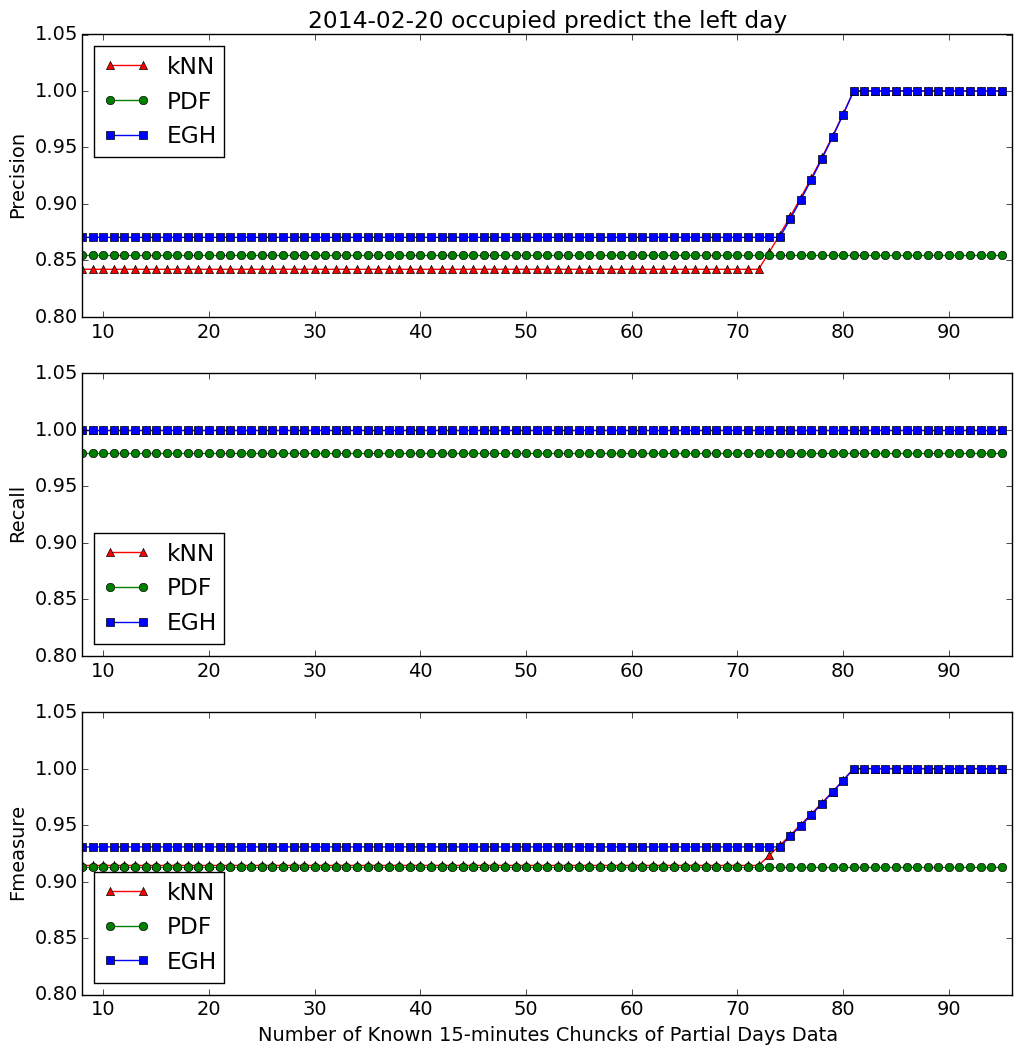
\includegraphics[width=0.7\textwidth]{adlfigs/study10person12014-02-20occupied.png}
\caption{Occupancy prediction precision, recall and f-measure comparison of three approaches 
of person1 on 02/20/2014 on Study10.}
\label{fig_study10}
\end{figure}
Figure~\ref{fig_study10} illustrates a person's occupancy prediction result in Study10.
There are three sub-figures. 
Each sub-figure describes the 
precision, recall, and f-measure 
of $person1$ on 02/20/2014. 
The blue line represents the mixture EGH model,
the green line represents the PDF model,
and the red line denotes the kNN model. 
The x-axis is the number of known 15-minute chunks of the test day. 
For instance, at $x=20$, 
we already know $20*15$ minutes' data 
and need to predict whether the home is occupied during the remaining $76$ chunks. 
The y-axis denotes the precision, recall and f-measure values 
in the three sub-figures from the top down. 
The first sub-figure shows that  
the mixEGH has the highest precision, recall and f-measure on test day 02/20/2014 
for occupancy prediction. The other two baseline approaches are comparable, except that kNN performs better than PDF 
when the person comes back home after slot 72. 
Looking into the original data, we find that person1 actually comes home later than usual 
in the training dataset. 
%In such case, mixture EGH performs best.  
%Figure \ref{fig_study10} (c) and (d) gives the occupancy and un-occupancy results 
%of person2 on 02/17/2014. 
%In such case, EGH mixture model performs best from the perspective of precision, recall and f-measure. 

\iffalse
Figure~\ref{fig_study14} (a) and (b) describe the case of person1 on 12/18/2013. 
Similar to Figure \ref{fig_study11} (a) and (b), 
mixture EGH model doesn't perform well before the person1 gets up 
and the reason keeps the same. 
The person1 slept late and some confused episodes are generated. 
Figure \ref{fig_study14} (c) and (d) describe the case of person1 on 12/19/2013. 
kNN performs better. MixtureEGH doesn't perform well because 12/19, 02/20 the person went out again after coming back and staying home for some time. However the training data don't include such case. 
\begin{figure}[h]
\centering
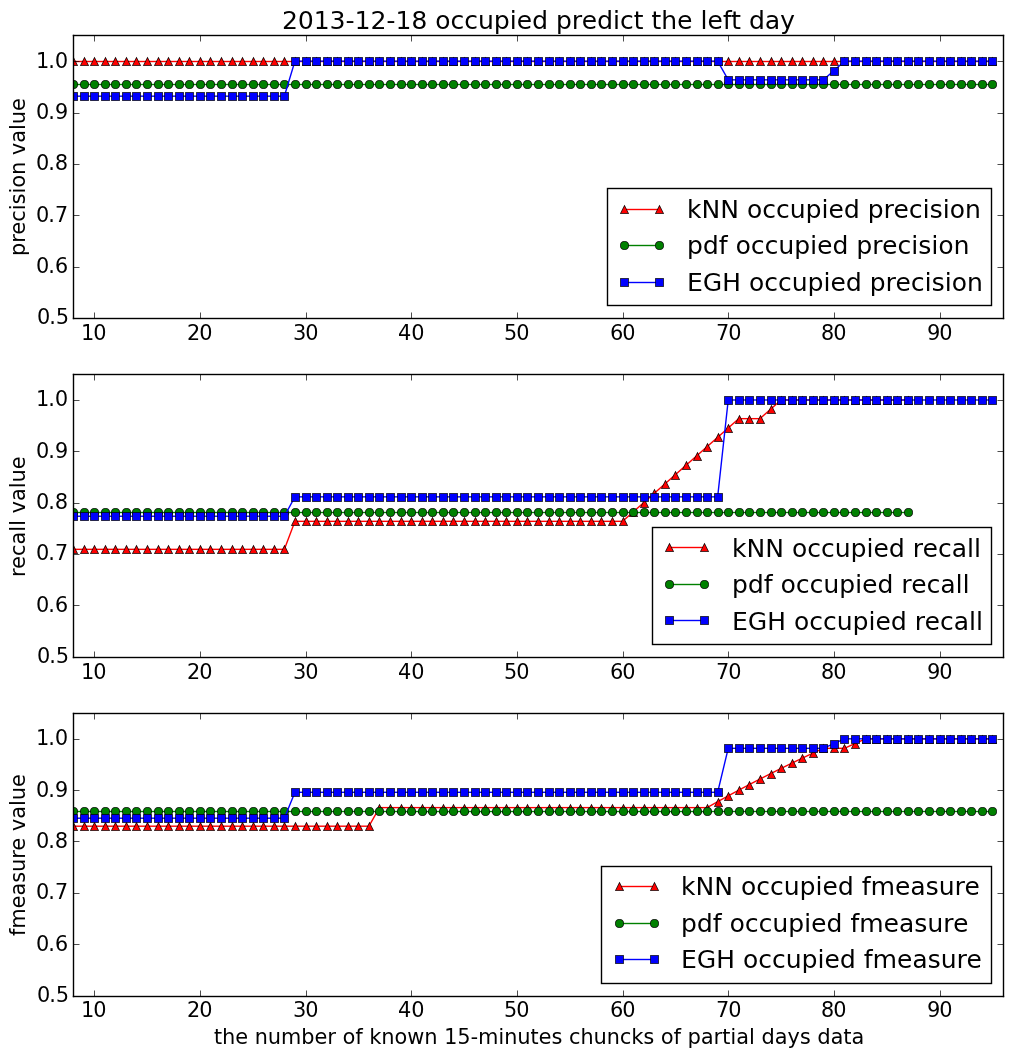
\includegraphics[width=0.5\textwidth]{adlfigs/study14person12013-12-18occupied.png} 
\caption{Study 14 Precision recall and f-measure comparison of three approaches.
person1 occupied 12/18/2014.}
\label{fig_study14}
\end{figure}
\fi


\subsection{Occupancy Prediction of Residential Buildings}
Based on individual prediction results, we deduce when a house is occupied
using logic OR operations on the prediction results of two persons. 
The whole house occupancy prediction results are listed in 
Table~\ref{tab_individualResults} and marked in bold. 
In Study10, the precision, recall, and fmeasure values of the whole house are 0.92, 0.92 and 0.91, respectively,  
which are higher than the values from the kNN approach of 0.91, 0.90 and 0.91, and of the SVR approach 0.79, 0.74 and 0.74. Similarly, the mixture EGH model outperforms kNN in Study11. 
Note that in Study 11 on 02/04/2015, 
EGH does not perform as well as kNN on individuals
but performs a little bit better than kNN, and much better than SVR in occupancy prediction of the whole house. 
The reason behind this is because the activities of the two people inside the home 
are not synchronized. The mixture EGH model can predict the 
occupancy for each person and grasp each person's activities more accurately. 
%When applying the logic OR operations on these two persons, 
%for whole-house occupancy prediction. 
\subsection{Limitations of Mixture EGH Model}
Although the temporal mixture EGH model performs well on the datasets Study10 and Study11, 
the same is not true for the dataset Study14. 
Table~\ref{tab_resultsLimitation} shows that, 
in Study14, 
the mixture EGH model works better for the individual and whole-house occupancy predictions on 12/18/2013 but not on 12/19/2013 or 12/20/2013. 
We check the activities of both individuals on these two days 
and find that both of them went out again 
after coming back and staying home for a while.
Since the episodes of going out after coming back home from work 
do not occur frequently, mixture EGH cannot detect this pattern. Thus the occupancy prediction probability of these events 
is completely missing. However kNN performs well because it leverages all the 
historical data; therefore, even if the abnormal event occurs once, 
this prediction approach incorporates it and obtains the average value. 
To relax the limitations of abnormal events, 
we propose a hybrid model for prediction;
when deploying this occupancy prediction in reality, 
for example for a prediction that is 30 minutes ahead, 
just 15 minutes before the prediction, if a person goes out again after coming back, 
the deployed system switches to the kNN approach rather than the mixture EGH model for prediction. In such cases, this hybrid model can always get the best prediction results. 

\begin{table*}[!t]
%\vspace{0.2cm}
\hfill
%\begin{minipage}[t]{1.0\linewidth}%

\caption{Precision Recall F-measure of Individual and Whole House Occupancy Prediction in Study 14.}
\label{tab_resultsLimitation}
%\tbl{Precision Recall F-measure of Individual and Whole House Occupancy Prediction in Study 14.\label{tab_resultsLimitation}}{
%\begin{center}
%\makebox[\textwidth]{
\centering
\small
\setlength\tabcolsep{2pt}
\begin{tabular} {|l|l|l|l|l|l|l|l|l|l|l|l|}
\hline
\multirow{2}{*}{Dataset}&\multirow{2}{*}{Date}&\multirow{2}{*}{Person} & \multicolumn{3}{|c|}{EGH}&\multicolumn{3}{|c|}{kNN} & \multicolumn{3}{|c|}{SVM} \\
\cline{4-12}
&&& precision & recall &fmeasure &precision & recall & fmeasure &precision & recall & fmeasure  \\
\hline
\multirow{3}{*}{study14}  & 12/18/2013 & person2&  \textbf{0.91} &  \textbf{0.91} &  \textbf{0.89} & 0.87 & 0.87 & 0.84 & 0.73 & 0.77 & 0.71\\
\cline{2-12}
& 12/18/2013 & person1&  \textbf{0.92} &  \textbf{0.92} &  \textbf{0.91} & 0.90 & 0.90 & 0.89 & 0.73 & 0.76 & 0.71 \\
\cline{2-12}
& 12/19/2014 & person2& 0.86 & 0.86 & 0.85  & \textbf{0.90} & \textbf{0.90} & \textbf{0.88} & 0.73 & 0.76 & 0.71\\
\cline{2-12}
& 12/19/2014 & person1& 0.85 & 0.84 & 0.84  & \textbf{0.86} & \textbf{0.86} & \textbf{0.85} & 0.73 & 0.76 & 0.71 \\
\cline{2-12}
& 12/20/2014 & person2& 0.92 & 0.94 & 0.92  & \textbf{0.98} & \textbf{0.97} & \textbf{0.97} & 0.75 & 0.79 & 0.75 \\
\cline{2-12}
& 12/20/2014 & person1& 0.90 & 0.91 & 0.90  & \textbf{0.95} & \textbf{0.95} & \textbf{0.95} & 0.75 & 0.79 & 0.75\\
\cline{2-12}
& 12/18/2013 & \textbf{wholehouse}&  \textbf{0.91}& \textbf{0.91} & \textbf{0.90} & 0.88	& 0.88 & 0.86 & 0.75 & 0.72 & 0.70 \\
\cline{2-12}
& 12/19/2013 & \textbf{wholehouse} & 0.841	& 0.845 & 0.838&  \textbf{0.848}& \textbf{0.853} & \textbf{0.842} & 0.79 & 0.74 & 0.74 \\
\cline{2-12}
& 12/20/2013 & \textbf{wholehouse} & 0.92	& 0.90 & 0.90&  \textbf{0.94}& \textbf{0.93} & \textbf{0.93} & 0.74 & 0.72 & 0.70 \\
\hline
\end{tabular}
%}
%\end{center}
%\end{minipage}%
%\hfill%
\end{table*}
\subsection{House Occupancy Prediction 30 Minutes Ahead with Hybrid Approach}
To preheat the house, we need to evaluate how much time in advance to automatically turn on/off HVAC, and the advance notice time estimation is given in~\cite{scott2011preheat}. 
Here we use prediction of 30 minutes ahead of time house occupancy. 
%because it is reasonable for preheating. 
We compare the receiver operating characteristic (ROC curve) of three approaches: mixture EGH model,  kNN, and a hybrid approach of the mixture EGH model and kNN. 
In this hybrid approach, 
we set mixture EGH results as the baseline, 
then replace the values of the mixture model by the values from kNN model 
in the following two situations: 
1) After a person comes back home; and 2) When the prediction probability of kNN is greater than 0.8. 
Figure~\ref{fig_rocresults_1}, ~\ref{fig_rocresults_2}, and~\ref{fig_rocresults_3} illustrate the ROC curve of the whole house occupancy prediction on 02/20/2014 of dataset Study10, 02/04/2014 of dataset Study 11 
and 12/20/2013 of dataset Study14, respectively.  
The red and green lines represents the kNN and mixture EGH models; 
the blue line denotes the hybrid approach. 
The ROC curves show that the hybrid approach always has the largest area, namely 
0.96, 0.92 and 0.92, 
which indicate that the hybrid approach always performs best. 
%\begin{figure}[h]
	\centering{
		\begin{tabular}{cccc}		
		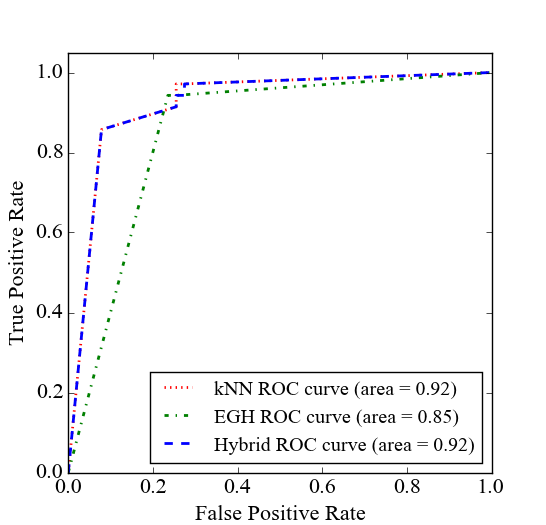
\includegraphics[width=0.5\textwidth]{adlfigs/study10ROC_02202014.png} &
		\tabular newline
		(a)\tabularnewline
		\end{tabular}
		}
	\caption{
	ROC curve of house occupancy prediction in Study10 (02/20/2014).}
	\label{fig_rocresults_1}
\end{figure}

\begin{figure}[h]
	\centering{
		\begin{tabular}{cccc}		
		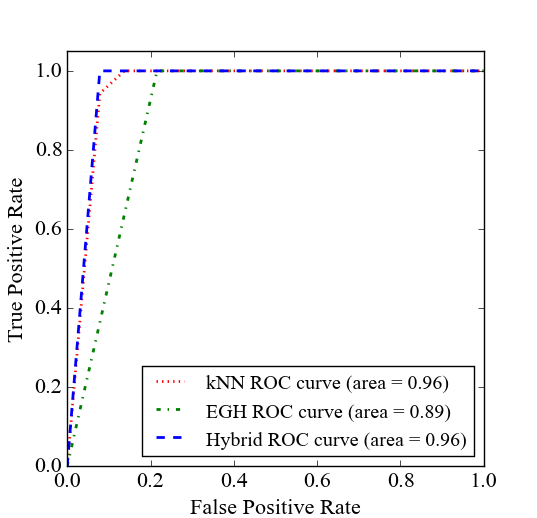
\includegraphics[width=0.5\textwidth]{adlfigs/study11ROC_02042014.png} &
		\tabularnewline
		((b)\tabularnewline
		\end{tabular}
		}
	\caption{
	ROC curve of house occupancy prediction in Study11 (02/04/2014).
}
	\label{fig_rocresults_2}
\end{figure}

\begin{figure}[h]
	\centering{
		\begin{tabular}{cccc}		
		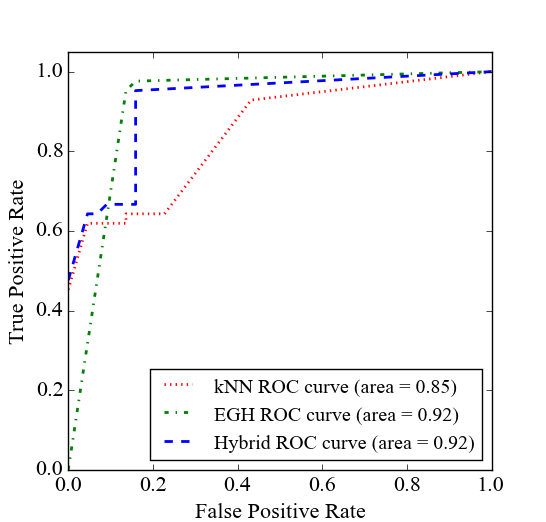
\includegraphics[width=0.5\textwidth]{adlfigs/study14ROC_12202013.png}
		\tabularnewline
		(c) \tabularnewline
		\end{tabular}
		}
	\caption{
	ROC curve of house occupancy prediction in (c) Study14 (12/20/2013).
}
	\label{fig_rocresults_3}
\end{figure}
\begin{figure}[h]
	\centering{
		\begin{tabular}{cccc}		
		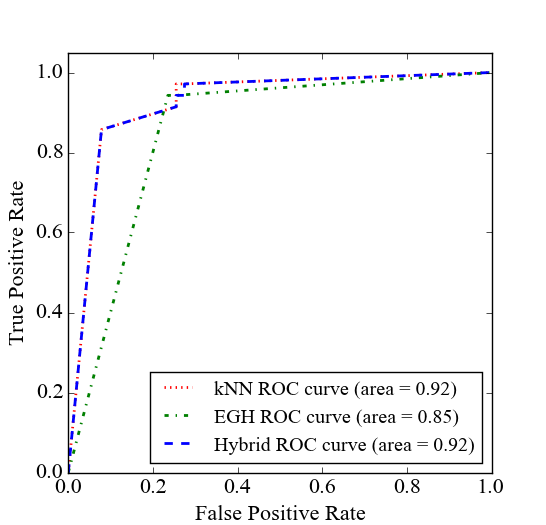
\includegraphics[width=0.6\textwidth]{adlfigs/study10ROC_02202014.png} &
		\tabularnewline
		(a)\tabularnewline
		\end{tabular}
		}
	\caption{
	ROC curve of house occupancy prediction in Study10 (02/20/2014).}
	\label{fig_rocresults_1}
\end{figure}

\begin{figure}[h]
	\centering{
		\begin{tabular}{cccc}		
		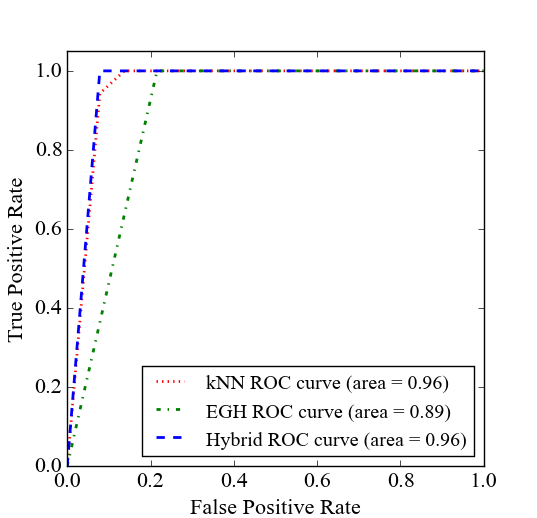
\includegraphics[width=0.6\textwidth]{adlfigs/study11ROC_02042014.png} &
		\tabularnewline
		((b)\tabularnewline
		\end{tabular}
		}
	\caption{
	ROC curve of house occupancy prediction in Study11 (02/04/2014).
}
	\label{fig_rocresults_2}
\end{figure}

\begin{figure}[h]
	\centering{
		\begin{tabular}{cccc}		
		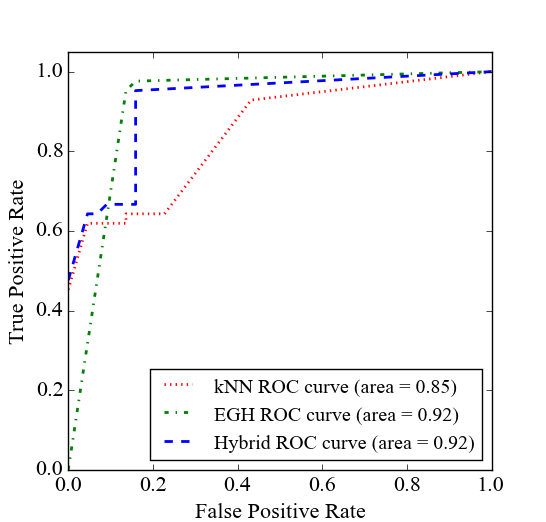
\includegraphics[width=0.6\textwidth]{adlfigs/study14ROC_12202013.png}
		\tabularnewline
		(c) \tabularnewline
		\end{tabular}
		}
	\caption{
	ROC curve of house occupancy prediction in (c) Study14 (12/20/2013).
}
	\label{fig_rocresults_3}
\end{figure}



%Also, we compare the 30 minutes whole house precision/recall/f-measure with the ROC curve, 
%the kNN ROC has a larger area even if EGH approach performs better on study10 and study11. 

%It depicts that ROC curve of mixture EGH model occupied larger area 0.92 than that from kNN approach 0.85. 
%We observe that although the precision/recall/fmeasure values are very close as in table~\ref{tab_individualResults}. 
%This hints that although the precision/recall/fmeasure results are competitive, 
%mixture EGH model can separate the occupancy and un-occupancy more sharply. 



%There are three test days in the dataset study14, 
%EGH outperforms kNN on the first day. 
%It's a tie on the second day. 
%The only exception on these datasets is the last day's experiment on study14, 
%kNN performs better because EGH mixture model currently
%only works on one-time even prediction. 



\section{Conclusion}
Residential occupancy prediction is a hot research topic supporting efforts to control HVAC systems more efficiently, 
with a consequent reduction in energy consumption. 
Increasing the accuracy of occupancy prediction allows these saving to be made 
without sacrificing the comfort of those living inside 
the home. 
In order to achieve the best prediction results, 
we propose integrating the mixture EGH model and 
kNN to create a new hybrid approach.

Our work differs from previous research based on the main contributions listed below:
\begin{enumerate}
\item We formulate the problem as one of temporal mining, 
where the activities inside the building are abstracted as episodes, 
and each episode is connected via an episode generative HMM model.
\item We mine the activity patterns according to the times and the gaps between them: 
both the duration of each type of 
activity, and the gap between two consecutive events are limited within an appropriate range. 
This range is extracted from historical data according to the day of the week and holidays.
\item Our hydrid prediction solution performs best for workday occupancy prediction: 
in the case of normal activities, a mixture EGH model is applied and
in the case of abnormal events, kNN is utilized,  
as this is generally considered a benchmark in occupancy prediction problems. 
\end{enumerate}
%In this paper, we propose the mixture EGH model and compare it with two other 
%benchmark models, probability density function and kNN approach. 
%The results show that it generally performs better than kNN to predict the 
%occupancy and un-occupancy states in the workdays. 
%The mixture model predicts well for the period of after person getting up and before person 
%going out. 
%The coefficient of the episode generative HMM models helps 
%predict the exact leaving time. 
%However in the case of abnormal events, 
%kNN performs good because it can average the 
%historical data. 
%Even if there is an abnormal day, 
%kNN can leverage it. 

In future work, we plan to continue working on improving holiday occupancy prediction. 
This is a  more intractable problem because 
the occupancy patterns for these days are completely different. 
For example, on certain days, a person may never leave the house. 
Therefore the occupancy prediction for holidays probably depends more on the date than on the indoor activities performed. 
We also plan to apply this new temporal mining approach to GPS datasets~\cite{koehler2013therml}
to test the effectiveness of occupancy prediction with different kinds of data. 
%%\section{Appendix}
%
%\renewcommand{\algorithmicrequire}{\textbf{Input:}}
%\renewcommand{\algorithmicensure}{\textbf{Output:}}

\begin{algorithm}
\caption{Gap Constraint Episode Mining on Dwelling Events}
\label{alg_episodeMiningConstraint_2e}
\SetKwData{Left}{left}\SetKwData{This}{this}\SetKwData{Up}{up}
\SetKwFunction{Union}{Union}\SetKwFunction{FindCompress}{FindCompress}
\SetKwInOut{Input}{input}\SetKwInOut{Output}{output}

%\begin{algorithmic} [1]
\Input {event stream $s=<(E_1, t_1^{start}, t_1^{end}), ..., (E_n, t_n^{start}, t_n^{end})>$;
events set $E$;
candidate of $N$-node episodes set C}
\Output {The set F of frequent serial episodes in C}
\For{ $A \in E$} {
$waits(A)= \phi$
}

\For{$\alpha \in C$} {
	$prev=\phi$
	\For{ $1 \leq i \leq N$ }{
		\emph{create $node$}; \\
		$node.visited=False$; $node.episode=\alpha$; $node.index=i$; $node.pre=pre$;$node.next=\phi$; \\
		\If{$i=1$}{
			$wait(\alpha[1]).add(node)$
		}
		\If{$prev!= \phi$}{
			$prev.next=node$
		}
	}
}
% there are four for cycles 
\For{$i=1:n$}{
	\For{ $node \in waits(E_i)$}{
	$accepted=false$;\\
	$\alpha=node.episode$; \\
	$j=node.index$; \\
	$tlist=node.list$; \\
	
	\If{$j<N$}{
		
		\For{$tval \in tlist$}{
			\If{$(t_i-tval.init) > \alpha.t_{high}[j]$}{
				$tlist.delete(tval)$ \\
				}
		}
	} % end of if j<N
	\eIf{$j=1$} {
		update $accepted=true$ \\
		$tval.init=t_i$ \\
		$tlist.add(tval)$ \\
		\If{$node.visited=false$}{
			update $node.visited=true$ \\
			$waits(\alpha[j+1]).add(node.next)$ \\
		}
	}
			%else
			{
				\For{$prev_{tval} \in node.pre.tlist$}{
					\eIf{$t_i-pre_{tval} \in (\alpha.t_{low}[j-1], \alpha_{high}[j-1])$}{
						Update $accepted=true$ \\
						update $tval.init=t_i$ \\
						$tlist.add(tval)$ \\
						\If{$node.visited=false$}{ 
							update $node.visited=true$ \\
							\If{$node.index\leq N-1$}{
								$waits(\alpha[j+1]).add(node.next)$ \\
							}
						}
					}
					%else
					{
						\If{$t_i-prev_{tval} > \alpha.t_{high}[j-1]$}{
 							$node.prev.tlist.remove(prev_{tval})$
						}
					}
			%		}
				} %forth for
			} % else
			
			
		%}% third for
	}
	\If{$accepted=true$ and $node.index=N$}{
		update $\alpha.freq=\alpha.freq+1$ \\
		set $temp=node$ \\
		\While{$temp!=\phi$} {
			update $temp.visited=false$ \\
			\If{$temp.index!=1$}{
		 		$waits(\alpha[temp.index]).remove(temp)$ \\
			}
			 update $temp=temp.next$
		}%end of while
	
	}%second for
} %first for
\For{$\alpha \in C$}{
	\If {$\alpha$.freq $>n*threshold$}{
		$F.add(\alpha)$ \\
	}
}
%\end{algorithmic}
\end{algorithm}

%\renewcommand{\algorithmicrequire}{\textbf{Input:}}
%\renewcommand{\algorithmicensure}{\textbf{Output:}}

\begin{algorithm}
\caption{Gap Constraint Episode Mining on Dwelling Events}
\label{alg_episodeMiningConstraint}
\begin{algorithmic} [1]
%\REQUIRE event stream $s=<(E_1, t_1^{start}, t_1^{end}), ..., (E_n, t_n^{start}, t_n^{end})>$;
%candidate of $N$-node episodes set C
%\ENSURE The set F of frequent serial episodes in C
\FORALL{ event type A}
\STATE Initialize $waits(A)= \phi$
\ENDFOR

\FORALL{$\alpha \in C$}
\STATE $prev=\phi$
\FOR{ $1 \leq i \leq N$ }
\STATE Create $node$ with $node.visited=False$; $node.episode=\alpha$; $node.index=i$; $node.pre=pre$;$node.next=\phi$
\IF{$i=1$}
\STATE Add $node$ to $wait(\alpha[1])$
\ENDIF

\IF{$prev!= \phi$}
\STATE $prev.next=node$
\ENDIF
\ENDFOR
\ENDFOR

\FOR{$i=1:n$}
\FORALL{ $node \in waits(E_i)$ }
\STATE set $accpeted=false$
\STATE set $\alpha=node.episode$
\STATE set $j=node.index$
\STATE set $tlist=node.list$

\IF{$j<N$}
\FORALL{$tval \in tlist$}
\IF{$(t_i-tval.init) > \alpha.t_{high}[j]$}
\STATE remove $tval$ from $tlist$
\ENDIF

\algstore{testcont}
\end{algorithmic}
\end{algorithm}

\begin{algorithm}[h]
\caption{Gap Constraint Episode Mining on Dwelling Events - Part 2}
\begin{algorithmic} [1]
\algrestore{testcont}


\IF{$j=1$}
\STATE update $accepted=true$
\STATE $tval.init=t_i$
\STATE add $tval$ to $tlist$
\IF{$node.visited=false$}
\STATE update $node.visited=true$
\STATE add $node.next$ to $waits(\alpha[j+1])$
\ENDIF
\ELSE
\FORALL{$prev_{tval} \in node.pre.tlist$}
\IF{$t_i-pre_{tval} \in (\alpha.t_{low}[j-1], \alpha_{high}[j-1])$}
\STATE Update $accepted=true$
\STATE update $tval.init=t_i$
\STATE add $tval$ to $tlist$
\IF{$node.visited=false$}
\STATE update $node.visited=true$
\IF{$node.index\leq N-1$}
\STATE add $node.next$ to $waits(\alpha[j+1])$
\ENDIF
\ENDIF
\ELSE
\IF{$t_i-prev_{tval} > \alpha.t_{high}[j-1]$}
\STATE remove $prev_{tval}$ from $node.prev.tlist$
\ENDIF
\ENDIF

\ENDFOR
\ENDIF

\ENDFOR
\ENDIF

\IF{$accepted=true$ and $node.index=N$}
\STATE update $\alpha.freq=\alpha.freq+1$
\STATE set $temp=node$
\WHILE{$temp!=\phi$}
\STATE update $temp.visited=false$
\IF{$temp.index!=1$}
\STATE remove $temp$ from $waits(\alpha[temp.index])$
\ENDIF
\STATE update $temp=temp.next$
\ENDWHILE
\ENDIF
\ENDFOR
\ENDFOR
%\STATE Output $F=\{\alpha \in C \} $ such that $ \alpha.freq \req n\lamba_{min} $
\end{algorithmic}
\end{algorithm}
% algorithm 03
\renewcommand{\algorithmicrequire}{\textbf{Input:}}
\renewcommand{\algorithmicensure}{\textbf{Output:}}

\begin{algorithm}
\caption{EM Algorithm for mixture EGH}
\label{alg3}
\begin{algorithmic} [1]
\REQUIRE day episode matrix, 
each element $e_{ij}$ records for each day whether an episode $j$ happens in day $i$;
frequent episodes $F=\{\alpha_1, ..., \alpha_J\}$;
symbol set $\varepsilon$;
threshold $\gamma$

\ENSURE the parameters for mixture EGH $\Lambda_Z=\{  (\Lambda_{\alpha_j}, \theta_j ) , j=1,...,J \}$


\STATE calculate the number of episodes J, and number of days K
\STATE calculate all $\eta$s' threshold value $mThreshold= \frac{M}{M+1}$

\COMMENT{initialize all the thetas to be $\frac{1}{J}$}
\COMMENT{calculate the total frequency for each episode over training time series}
\COMMENT{ calculate the $eta$ value}
\FOR{$0 \leq j \leq J$}
\STATE $\theta[j]= 1/J$
\STATE $episodeFreq[j] = \sum_i^K e_{ij}$
\ENDFOR

\STATE select those frequent episodes starting with 'S' and ending with 'Z' and separate these 
episodes by workday or holiday

\COMMENT {calculate $eta$ for each episode} 
\FOR{$0 \leq j \leq J$}
\STATE $\eta[j]= 1-episodeLen[j]*episodeLen/T$
\ENDFOR

\COMMENT{likelihood prediction of each episode $j$ in the $k$th day}

\FOR{$0 \leq i \leq K$}
\FOR{$0 \leq j \leq J$}
\STATE $likelihood_{ij} = \frac{1-\eta[j]}{\eta[j]/M} ^ {episodeLen[j]*e_{ij}}$
\ENDFOR
\ENDFOR

\COMMENT{calculate the obj value based on J, K, $likelihood_{ij}$ and $\theta$}
\WHILE{$newObj- obj > \gamma$}
\STATE $\theta_{new}=[]$
\FOR{$0 \le l \le J$}
\STATE $temp=0$
\FOR{$0 \le j \le K$}
%\COMMENT{calcuate the new likelihood with Bayes rules}
\STATE $temp = temp+ \frac{\theta_l*likelihood_{il}}{ \sum_0^J { \theta_j*likelihood_{ij}}}$

\ENDFOR
\STATE $\theta_{new}[l] = temp/K $
\ENDFOR

\STATE calculate the newObj
\IF{$newObj-obj > \gamma$}
\STATE $obj=newObj$
\STATE $\theta_{new} = \theta$
\ENDIF

\ENDWHILE

\STATE Output $\Lambda_Z=\{  (\Lambda_{\alpha_j}, \theta_j ) , j=1,...,J \}$

\end{algorithmic}
\end{algorithm} 



\bibliographystyle{ACM-Reference-Format}
\bibliography{references} 

\end{document}
